\documentclass[11pt,a4paper]{report}

\usepackage{fullpage}
\usepackage{fancyhdr}
\usepackage{lastpage}
\usepackage{mathtools}
\usepackage{gensymb}
\usepackage{fontspec}
\usepackage{color}
\usepackage{graphicx}
\usepackage{wrapfig}
\usepackage{tabularx}
\usepackage{hyperref}
\usepackage[french]{babel}
\usepackage{indentfirst}
\usepackage{multicol}
%\usepackage{float}
\usepackage{mdwlist}
%\usepackage{bnf}
\usepackage{listliketab}
\usepackage[export]{adjustbox}
\usepackage{subfigure}


% for languages codes
\usepackage{xcolor}
\usepackage{listings}
\renewcommand{\lstlistingname}{Extrait de code}
\lstset{basicstyle=\ttfamily,
  showstringspaces=false,
  commentstyle=\color{gray},
  keywordstyle=\color{blue}
}
% https://tex.stackexchange.com/questions/89574/language-option-supported-in-listings
\lstdefinelanguage{javascript}{
  keywords={typeof, new, true, false, catch, function, return, null, catch, switch, var, if, in, while, do, else, case, break},
  keywordstyle=\color{blue}\bfseries,
  ndkeywords={class, export, boolean, throw, implements, import, this},
  ndkeywordstyle=\color{darkgray}\bfseries,
  identifierstyle=\color{black},
  sensitive=false,
  comment=[l]{//},
  morecomment=[s]{/*}{*/},
  commentstyle=\color{gray}\ttfamily,
  stringstyle=\color{green}\ttfamily,
  morestring=[b]',
  morestring=[b]"
}


\newcommand\vartitle{Étude sur l'apprentissage par renforcement dans les jeux \\Projet de Bachelor 2018 - hepia}
\newcommand\varauthor{Étudiant: Federico Pfeiffer \\Professeur: Guido Bologna}
\newcommand\vardate{\today}

\title{\vartitle}
\author{\varauthor}
\date{\vardate}

% page layout
\pagestyle{fancyplain}
\lhead[\vartitle]{\vartitle}
\chead[]{}
\rhead[\varauthor]{\varauthor}
\lfoot[]{}
\cfoot[\thepage\ of \pageref{LastPage}]{\thepage\ of \pageref{LastPage}}
\rfoot[]{}

\renewcommand{\headrulewidth}{0.2mm}
\renewcommand{\footrulewidth}{0mm}

\setlength{\headsep}{40pt}
\setlength{\voffset}{0cm}
\setlength{\topmargin}{-1.7cm}
\setlength{\textheight}{730pt}

\setlength{\columnsep}{30pt}

\setlength{\parindent}{0mm}
\setlength{\parskip}{2mm}

% only chapters / sections / subsections are numbered 
\setcounter{secnumdepth}{2}

% only chapters / sections are in table of contents
%\setcounter{tocdepth}{1}



\hypersetup{
  hidelinks,
  pdfstartview={FitV},
  pdftitle={\vartitle},
  pdfauthor={\varauthor}
}

\begin{document}

  \begin{titlepage}
    \maketitle

    \thispagestyle{empty}

    \begin{abstract}
    // TODO
    \end{abstract}

%    \vspace{1cm}

  \end{titlepage}
  
  \newpage
  
  \tableofcontents
  
  \newpage

  \chapter{Introduction}
  
  \section{Contexte}
  
  \par L'apprentissage par renforcement est une branche d'intelligence artificielle connaissant un essor depuis quelques années, et qui a permis des avancées technologiques telles que la voiture autonome, le logiciel "AlphaGo" de Google réussissant à battre le champion du monde de Go, ou encore la création de robots capables d'apprendre à se mouvoir sans intervention humaine. Le champ d'application est vaste, et est actuellement sujet à de nombreuses recherches pour découvrir de nouveaux champs d'applications. 
  
  \par J'ai profité du travail de Bachelor afin d'étudier par la pratique l'apprentissage par renforcement. Pour ce faire, un environnement de jeu a été créé pour faire évoluer un agent dans celui-ci. L'étude des réseaux de neurones artificiels a également été nécessaire étant donné qu'une grande partie des algorithmes d'apprentissage par renforcement utilisent de tels réseaux de neurones. 
  
  \section{Objectifs}
  
  \par Les objectifs de ce présent travail de bachelor sont les suivants: 
  
  \renewcommand{\labelitemi}{\textbullet}
  \begin{itemize}
  \item Comprendre les modèles de réseaux de neurones artificiels standards et profonds
  \item Comprendre les concepts de l'apprentissage par renforcement
  \item Comprendre et utiliser au moins un "framework" pour l’utilisation de l'apprentissage par renforcement
  \item Construire un jeu avec un agent qui apprend par renforcement
  \item Analyse des résultats 
  \item Rédaction du rapport
  \end{itemize}
  
  \section{Réalisation}
  
  \par Le jeu dans lequel l'agent évolue est le suivant: un agent (en bleu) doit éviter des ennemis représentés en rouge, tout en récupérant de la nourriture (en vert). Au fur et à mesure que l'agent avance, l'endurance de l'agent faibli (le diamètre de l'agent diminue). Si l'endurance de l'agent est trop faible, le jeu se termine. Si l'agent se fait attraper par un ennemi, le jeu est également terminé. Si l'agent atteint la nourriture, son endurance est remise au maximum, et une nouvelle nourriture est placée aléatoirement dans le jeu. Le but de l'agent est de tenir un maximum de temps sans que le jeu se termine. Les actions possibles dans l'environnement sont d'avancer dans une direction des points cardinaux (N, NE, E, SE, S, SO, O, NE), ou ne rien faire. Le nombre d'actions possibles équivaut donc à neuf. 
  
   \begin{figure}[!h]
   \center
   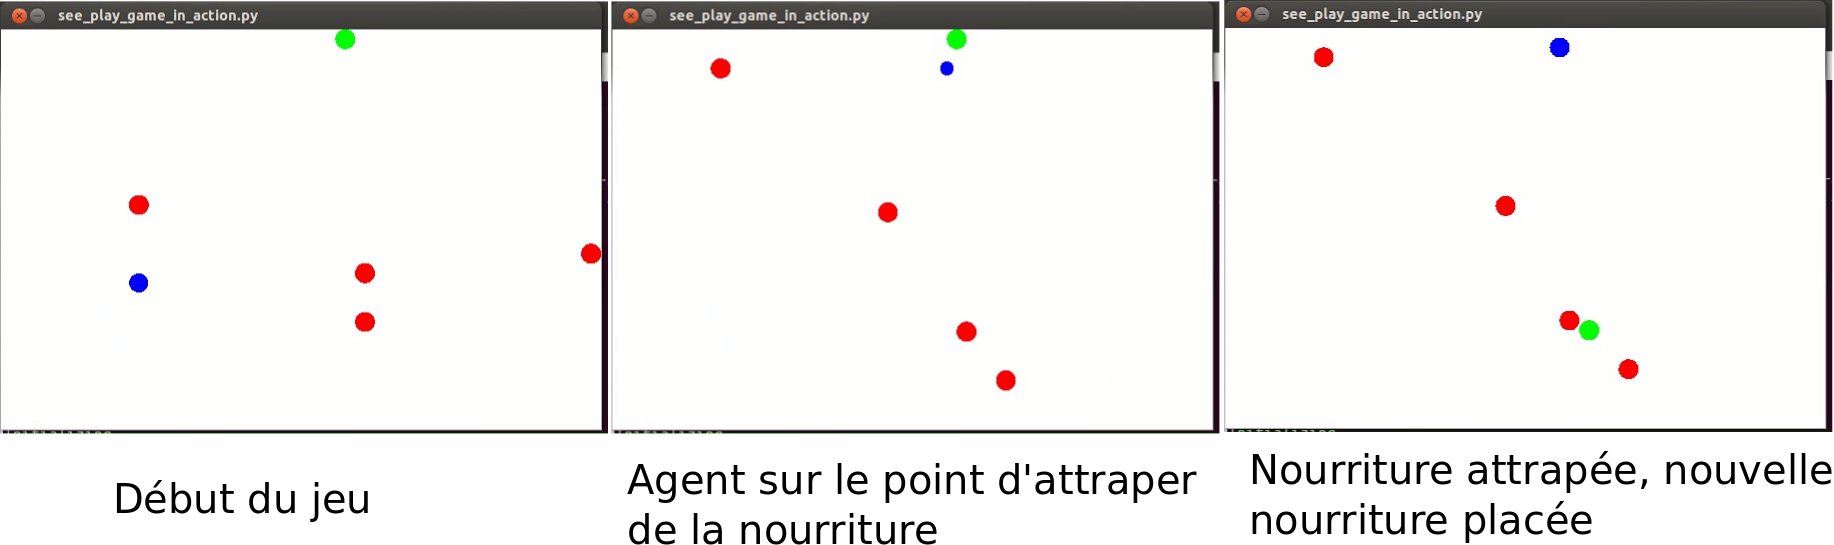
\includegraphics[scale=0.2]{ressources/presentation_jeu.png}
   \caption{Présentation de l'environnement (Jeu)}
   \end{figure} 
  
  \par Afin de faciliter l'apprentissage, ce dernier a été divisé en 3 parties: 
  
  \begin{enumerate} 
  \item Apprendre à éviter les ennemis (sans nourriture)
  \item Apprendre à attraper la nourriture (sans ennemis)
  \item Une fois les deux premières compétences apprises, l'agent doit ensuite apprendre à jongler entre les deux compétences afin de jouer convenablement au jeu. 
  \end{enumerate}
  
  \par Cela implique les contraintes suivantes: 
  
  \begin{itemize}
  \item L'environnement (jeu) doit être configurable pour qu'il être utilisé indépendamment avec uniquement des ennemis, que de la nourriture, ou les deux en même temps. 
  \item L'agent doit être implémenté de manière générique, de sorte à ce qu'il puisse apprendre les connaissances indépendamment. (éviter les ennemis, attraper la nourriture, ou les deux en même temps). 
  \item Une fois des connaissances apprises, l'on doit pouvoir les sauvegarder afin de pouvoir les réutiliser pour la suite de l'apprentissage: une fois que l'agent a appris à éviter les ennemis ou attraper de la nourriture, il faut pouvoir faire en sorte de réutiliser ces compétences sans avoir à les réapprendre à chaque fois que le programme démarre. 
  \end{itemize}
  
  \chapter{Théorie}
  
  \section{Définitions}
  
  \subsubsection{Apprentissage par renforcement}  
  
    \par L'apprentissage par renforcement consiste à considérer un agent autonome évoluant dans un environnement donné. La seule chose que connaît l'agent sont les différentes actions qu'il peut effectuer au sein de son environnement. Le but de l'agent est d'obtenir un score maximal par le biais de récompenses vis à vis des actions qu'il a entrepris.
    
    \par Au début, l'agent choisit les actions de manière aléatoire, et on lui indique si l'action qu'il a entrepris lui confère une récompense, un malus, ou pas de retour particulier. Si l'état terminal est atteint, l'environnement est remis à zéro et l'agent continue ses expériences depuis cet état initial. L'agent peut ainsi "apprendre par la pratique", les actions à entreprendre en fonction de l'état où il se trouve, dans le but de maximiser le score.
  
  \subsubsection{Agent}
  
    \par Un agent est un programme informatique autonome, ou une partie d'un programme qui est autonome, c'est à dire qu'il ne dépend pas d'interventions extérieures pour évoluer. (Il ne doit pas rester bloqué en attente d'une intervention humaine). 
    
    \par Les entrées (input) de l'agent permettent de percevoir l'environnement dans lequel l'agent évolue. Les sorties (output) de l'agent sont les actions choisies par l'agent pour influer sur l'environnement dans lequel il évolue. Il n'y a pas d'autres entrées/sorties. Toute la logique applicative liée à l'agent est donc implémentée au sein de l'agent. La seule chose avec laquelle communique l'agent est donc l'environnement externe, par le biais de "capteurs" ou autres "sens" au terme "biologique". Il est important de signaler que l'agent n'a pas forcément conscience de l'état complet de l'environnement. La représentation de l'environnement que l'agent se fait dépend donc des capteurs qu'il détient. 
   
  \subsubsection{Environnement}
  
    \par L'environnement est le monde dans lequel l'agent évolue et dans lequel l'agent, de par ses actions, modifie l'état de l'environnement. L'environnement est séparé de l'agent, et le seul lien entre ces derniers sont les \textit{inputs} de l'agent, c'est à dire les capteurs par lesquels l'agent peut percevoir l'environnement, et les \textit{outputs} de l'agent, c'est à dire les différentes actions que l'agent a pour influer sur l'environnement. 
    
  \subsubsection{État et état terminal}
  
    \par Un état est une photo instantanée du monde perçu par l'agent. Un état comprend l'état de l'environnement ainsi que l'état de l'agent. Un état terminal représente un état dans lequel l'agent n'a plus d'actions à effectuer. Étant donné qu'il n'y a plus d'actions à effectuer, l'environnement peut alors être "remis à zéro" afin que l'agent puisse recommencer à évoluer. 
  
   \subsubsection{Action et récompense}
  
    \par Chaque action mène à un changement d'état. Une action est la seule possibilité pour un agent d'influencer l'environnement dans lequel il évolue. C'est aussi la seule manière pour un agent de savoir si l'action qu'il a entrepris est bonne, mauvaise ou "sans effet". Pour chaque action, l'agent reçoit donc une récompense (bonne, mauvaise ou neutre). Si la récompense est "bonne", l'agent reçoit un score positif; si l'action est "mauvaise", l'agent reçoit une récompense négative. L'agent peut alors ajuster son expérience dans le but de favoriser les actions menant à maximiser un score positif, ou minimiser un score négatif.
    
    \par Si la récompense est neutre, l'agent enregistre néanmoins l'action qu'il a entrepris au cas où l'action neutre même à futur état permettant un score positif ou négatif. Si l'agent est un joueur d'échec et que l'action qu'il entreprend ne permet pas de gagner, il est quand même important d'enregistrer l'état/action vécu si jamais cela l’emmène par la suite dans un état/action où il gagne ou perd. De même, si une voiture doit tourner à gauche et qu'elle continue tout droit pendant une fraction de seconde, elle doit pouvoir savoir si le fait de tourner à gauche la fraction de seconde d'après l'amènera à une sortie de route, ou si elle peut quand même tourner à gauche sans sortir de route. 
    
    \par L'important pour l'agent est de pouvoir enregistrer les actions prises d'une manière où d'une autre, en vue de savoir si cette action mène plutôt à un échec, une réussite, ou à un état neutre. 
    
    \begin{figure}[!h]
    \center
    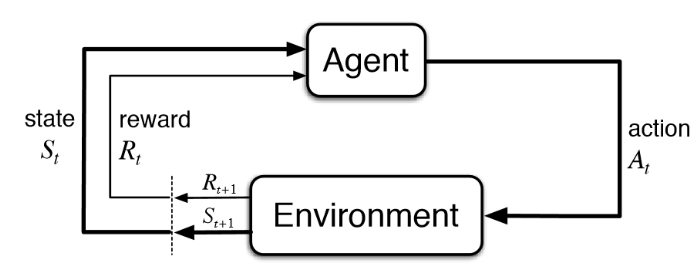
\includegraphics[scale=0.5]{ressources/shema_agent_environnement.png}
    \caption{Action et récompenses}
    \end{figure} 
    
  \subsubsection{Épisode}
  
    \par Un épisode commence depuis l'état initial (environnement mis à zéro) et termine à un état terminal. Lorsque l'agent atteint un état terminal, l'environnement est réinitialisé et l'agent recommence un nouvel épisode. L'agent enregistre chaque récompense durant toute la durée de l'épisode afin de connaître le score total que l'agent a eu pendant l'épisode.
    
  \section{Notions de base}
  
  \subsection{Fonctionnement général de l'apprentissage par renforcement}
  
    \par L'apprentissage par renforcement consiste à donner une récompense à un agent lorsque ce dernier parvient à effectuer une tâche demandée, ou lorsqu'il s'en approche. De la même manière, l'agent reçoit un malus lorsque ce dernier s'éloigne de la tâche demandée. Le but de l'agent est d'obtenir un maximum de récompense. De cette manière, le comportement de l'agent est influencé par les récompenses et malus qu'il reçoit. Au fur et à mesure que l'agent effectue des actions et reçoit des récompenses/malus, ce dernier tend à renforcer un comportement menant à un maximum de récompenses, et éviter les actions menant à des malus. À noter qu'à partir de maintenant nous ne parlerons que de récompenses: un malus sera simplement traduit par une récompense négative. 
  
    \par Plus concrètement, l'agent commence par effectuer des actions aléatoires et reçoit une récompense / malus pour chaque action effectuée. Pour chaque action commise, l'agent enregistre l'état $S$ dans lequel il se trouvait, l'action effectuée, la récompense/malus reçue  et l'état $S'$ dans lequel il se retrouve suite à l'action. Si l'agent se retrouve dans un état terminal, l'environnement est réinitialisé mais l'agent garde en mémoire les actions / états / récompenses vécus. À une fréquence définie par le développeur, l'agent passe par une phase d'ajustement \textit{(training)} où il parcourt tous les actions / états / récompenses vécus de sorte à ajuster son comportement (actions choisies) lors des états futurs qu'il rencontrera, dans le but de maximiser les récompenses. 

  \subsection{Valeur d'un état}
  
    \par Jusqu'à la fin du chapitre, nous définirons le score d'un épisode par la somme des récompenses obtenues au cours des actions effectuées. Le but de l'agent est d'obtenir le meilleur score possible, et de retenir les états par lesquels il est passé afin d'obtenir ce meilleur score. (Et également de retenir les états par lesquels il est passé qu'il l'ont mené à un mauvais score). 
    
    \par Afin d'apprendre à choisir les bonnes actions à effectuer en fonction de l'état où l'agent se trouve, ce dernier a pour but d'apprendre la valeur de chaque état qu'il rencontre: un état qui le rapproche d'un meilleur score a une meilleure valeur qu'un état qui l'éloigne d'un meilleur score. 
    
    \par L'enjeu est donc de trouver une manière d'attribuer une valeur à chaque état en fonction des états qui vont suivre, afin de choisir l'action appropriée menant à un meilleur état. Prenons l'exemple (arbitraire) comprenant 2 épisodes, avec un état initial s0 \textit{(s pour state)}: 
    
    \begin{figure}[!h]
    \center
    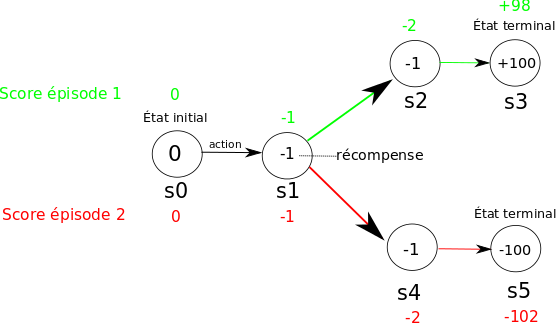
\includegraphics[scale=0.60]{ressources/introduction_function_value.png}
    \caption{Valeur d'un état: introduction 1}
    \end{figure} 
    
    \par Dans le premier épisode, l'agent commence à l'état s0 (état initial), puis choisit les actions passant par s1, s2 et s3. s3 étant un état terminal, l'épisode 1 s'arrête et l'agent obtient comme score +98 (qui est la somme des récompenses obtenues pendant son épisode). Dans le deuxième épisode, l'agent commence à l'état s0 (état initial), puis choisit les actions passant par s1, s4 et s5. s5 étant un état terminal, l'épisode 2 s'arrête et l'agent obtient un score de -102 pour le deuxième épisode. 
    
    \par Comment pourrions-nous donc attribuer une valeur à chaque état? Intuitivement, nous concluons qu'il est nécessaire d'attribuer une valeur à chaque état une fois qu'un épisode est terminé. En effet, une fois l'épisode terminé, nous pouvons évaluer chacune des actions prises par l'agent, étant donné que nous savons si les actions effectuées ont mené à l'état terminal voulu. Une première idée serait donc d'attribuer à chaque état la récompense finale auquel l'état peut mener. Si un état mène à deux récompenses différentes, nous pouvons par exemple attribuer la valeur de l'état en faisant la somme des deux récompenses auxquels l'état peut mener. 
    
    \begin{figure}[!h]
    \center
    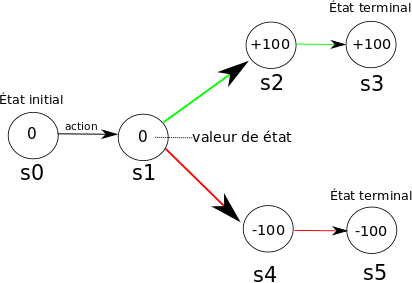
\includegraphics[scale=0.60]{ressources/introduction_function_value_2.png}
    \caption{Valeur d'un état: introduction 2}
    \end{figure}
    
    \par Après avoir effectué sa phase d'ajustement \textit{(training)} dans le but de connaître la valeur de chaque état (phase d'apprentissage), l'agent peut ensuite savoir que depuis l'état s1, il est préférable de choisir l'action menant à l'état s2, étant donné qu'un meilleur score l'attend.
    
\subsubsection{Discount factor ($\gamma$)}
  
    \par Le problème de la méthode précédente pour attribuer une valeur à un état est qu'on ne tient pas compte de la distance à laquelle se trouve la récompense finale.\\
    En prenant l'exemple suivant, il serait préférable pour l'agent de passer directement à s3 depuis s1. (L'agent a meilleur temps d'effectuer l'action qui le mène le plus rapidement à l'état menant à une forte récompense). Or, l'agent n'a pas de moyen de savoir qu'il a meilleur temps de passer directement par s3:
    
    \begin{figure}[!h]
    \center
    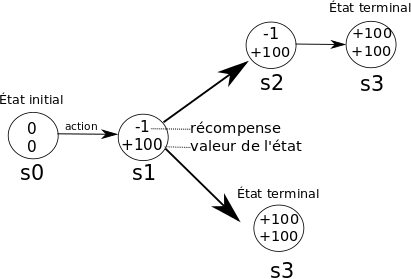
\includegraphics[scale=0.60]{ressources/introduction_function_value_3.png}
    \caption{Valeur d'un état: introduction sans discount factor}
    \end{figure}
    
    \par Une solution pour palier à ce problème est de calculer la valeur d'un état en ajoutant un coefficient nommé \textit{discount factor} $\gamma$ de cette manière: $V(s_t) = \gamma V(s_{t+1})$ avec $\gamma \in [0,1]$. En prenant $\gamma = 0.9$, on parvient à attribuer une valeur à chaque état qui inclut cette notion de distance envers la récompense la plus forte. Depuis s1, l'agent va donc tendre vers s3 directement car la valeur de s3 est plus grande que s2.
    
    \begin{figure}[!h]
    \center
    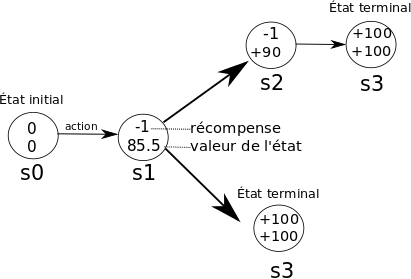
\includegraphics[scale=0.60]{ressources/introduction_function_value_4.png}
    \caption{Valeur d'un état: introduction avec discount factor}
    \end{figure} 
    
  \subsection{V(s): Équation de Bellman}
  
    \par La fonction $V(s) = \gamma V(s_{t+1})$ est incomplète. La version formelle vient de l'équation de Bellman. Elle prends en compte plusieurs notions  supplémentaires: 
    
    \par Elle prends en compte la récompense reçue à chaque état, ce qui donne \\ $V(s_t) = r + \gamma V(S_{t+1})$
    
    \par Aussi, il est possible qu'un environnement soit fait de telle sorte qu'une transition d'un état à un autre ne soit pas déterministe. Par exemple, si un agent choisit une action menant à un état $S'$, on peut imaginer que l'environnement aie un comportement aléatoire menant l'agent à un état qui n'était pas prévu par l'agent. (dans l'exemple d'une voiture autonome, le fait de voir un enfant jouer sur un trottoir n'implique pas forcément que celui-ci reste sur le trottoir). Pour un état $s_t$, il faudrait pouvoir multiplier la probabilité de se retrouver dans un état $s_{t+1}$, et recevoir une récompense $r$ après avoir fait une action $a$. En d'autres termes, pour un état $s_t$, il faut évaluer tous les états $s_{t+1}$ et toutes les récompenses $r$, et en calculer la probabilité. \\
    La fonction V(s) devient $$\sum_{s_{t+1}}\sum_rp(s_{t+1},r\ |s_t,a)\left\{r+\gamma V(s_{t+1})\right\}$$
    
    \par Enfin, il se peut que pour un certain état, l'agent aie une certaine probabilité de choisir une certaine action. (Il peut par exemple connaître la meilleur action à entreprendre, mais il a une politique d'avoir 10\% de probabilité de faire une action aléatoire dans le but d'explorer certaines actions). La fonction est alors agrémentée du terme suivant: $\sum_a\pi(a|s)$. Le $\pi$ représente la politique de l'agent.
    
    \par Ainsi, l'équation de Bellman indique que la valeur d'un état peut se calculer de la manière suivante: 
    
    $$V_\pi(s) = \sum_a\pi(a|s)\sum_{s'}\sum_rp(s',r\ |s,a)\left\{r+\gamma V_\pi(s')\right\}$$
    
    \par Le terme $\pi(a|s)$ représente la probabilité de choisir une action $a$ étant donné l'état $s$, suivant une politique $\pi$. (Dans le cas où la politique de l'agent est de choisir une action aléatoire tous les 10\% par exemple). Si l'agent a une politique visant à ne choisir que la meilleure action et que le choix de cette action n'est pas probabiliste, ce terme vaut simplement 1. De même, si l'agent n'a qu'une action possible pour un certain état $s$, le terme $\sum_a\pi(a|s)$ équivaut à $\pi(a|s)$
    
    \par Le terme $p(s',r\ |s,a)$ représente, depuis un état $s$, la probabilité de se retrouver dans l'état suivant $s'$ et de gagner la récompense $r$, ayant choisi l'action $a$. Pour connaître la valeur de l'état $s$, il faut donc pouvoir envisager tous les états $s'$ possibles, et toutes les récompenses $r$ en choisissant une action $a$. C'est pour cela que l'on "itère" en faisant la somme de tous les $p(s',r\ |s,a)$ en parcourant tous les états $s'$ possibles et toutes les récompenses $r$ possibles depuis un état $s$. D'où les deux sommes $\sum_{s'}\sum_r$ devant $p(s',r\ |s,a)$:  $\sum_{s'}\sum_rp(s',r\ |s,a)$
    
    \par L'équation de Bellman peut être lue de la manière suivante: depuis un état $s$, on itère toutes les actions possibles depuis cet état. Dans cette itération, on itère toutes les récompenses possibles et tous les états $s'$ qui découlent en choisissant l'action $a$. A chaque itération, on multiplie la probabilité $\pi(a|s)$ à la probabilité $p(s',r\ |s,a)$ et multiplie à la $\left\{r+\gamma V_\pi(s')\right\}$
    
    $$V_\pi(s) = \sum_a\pi(a|s)\sum_{s'}\sum_rp(s',r\ |s,a)\left\{r+\gamma V_\pi(s')\right\}$$
    
    \par Dans ce projet de bachelor, nous considérerons l'environnement déterministe, ce qui réduit l'équation de Bellman à ceci: 
    
    $$V_\pi(s) = \sum_a\pi(a|s)\left\{r+\gamma V_\pi(s')\right\}$$

    
  \subsection{Apprentissage par renforcement: pseudo code}
  
  \par Maintenant que nous connaissons comment attribuer une valeur à chaque état, nous pouvons imaginer un premier pseudo-code permettant à un agent d'apprendre à évoluer dans un environnement. Le problème de cette équation est qu'elle part du principe que nous connaissons tous les états et actions possibles. Il faut donc procéder de manière itérative jusqu'à ce que la valeur d'un état converge vers une valeur fixe. Nous nous arrêtons lorsque toutes les valeurs des états semblent avoir été calculées:  
  
   \begin{lstlisting}[language=python]
 
  # phase d'apprentissage
  world = new World()
  agent = new Agent()
  gamma = 0.9
  
  max_divergence = 0.1
  divergence = inf
  while divergence > max_divergence:
    for state in world.get_all_states():
      for action in world.get_possible_actions(state):
        reward, next_state = world.do_action(state, action)
        old_v = agent.V[state]
        agent.V[state] = reward + gamma * agent.V[next_state]
        divergence = max(divergence, abs(old_v-agent.V[state]))
        
  # phase une fois l'apprentissage effectué
  state = world.reset()
  while not world.is_in_terminal_state():
    action = agent.choose_action_to_best_state(state)
    state = world.do_action(action)
        
   \end{lstlisting}
  
  \par Supposer que l'on doive connaître tous les états et actions possibles pose évidemment problème dans le cas de l'apprentissage par renforcement, étant donné que l'agent doit apprendre en explorant lui-même à travers les actions qu'il entreprend. Pour des raisons de temps de calcul, nous ne souhaitons pas explorer toutes les actions possibles, mais souhaitons explorer que celles qui nous semblent nous mener à un meilleur comportement de l'agent. Heureusement, des algorithmes ont été mis en place afin de pouvoir estimer correctement la fonction de Bellman ($V(s)$) sans avoir à tout explorer, permettant ainsi à l'agent de pouvoir estimer raisonnablement la valeur de l'état dans lequel il se trouve, et choisir l'action adéquate pour maximiser son score. 
    
  \section{Algorithme Q-Learning}
  
  \subsection{Explore vs Exploit} 
  
    \par Dans la précédente section, nous avons vu un algorithme permettant d'évaluer V(s) en supposant que l'on connaisse tous les états, actions et récompenses possibles suivant l'environnement donné. Dans la majorité des cas, il n'est évidemment pas possible de connaître toutes ces valeurs à l'avance. Il convient donc d'utiliser l'agent de sorte à ce qu'il explore de lui même toutes ces différentes valeurs dans le but d'estimer correctement la fonction V(s).     
    
    \par Au fur et à mesure que l'agent explore les actions, la fonction V(s) va petit à petit atteindre une estimation correcte, et l'agent va petit à petit connaître les meilleurs états à rencontrer, ou les meilleures actions à effectuer pour chaque état. 
    
    \par Comment savoir si l'agent dispose de connaissances suffisantes pour arrêter d'explorer/tester des actions? A quel moment l'agent doit-il utiliser la connaissance qu'il dispose de V(s)? Une solution est d'effectuer une action aléatoire avec une probabilité $\epsilon$. La valeur de $\epsilon$ peut varier en fonction du temps selon ce qu'a choisit le programmeur. 
  
  \subsection{Valeur d'un état avec Q(s,a)}
  
    \par Utiliser V(s) pour attribuer une valeur à chaque état peut s'avérer limitant: on n'enregistre finalement que la valeur d'un état en fonction de l'état en question. Au lieu d'attribuer une valeur à un état, nous pourrions attribuer une valeur à un couple état/action effectué. 
    
    \par La fonction attribuant une valeur à un couple état/action s'appelle la fonction Q value, ou Q(s,a), et peut être représentée de la sorte, ressemblant fortement à V(s): 
        
    \begin{eqnarray}
      V_\pi(s) &=& \sum_a\pi(a|s)\sum_{s'}\sum_rp(s',r\ |s,a)\left\{r+\gamma V_\pi(s')\right\} \\
      Q_\pi(s,a) &=& \sum_{s'}\sum_rp(s',r\ |s,a)\left\{r+\gamma Q_\pi(s',a')\right\}
    \end{eqnarray}
    
    \par Comme indiqué plus haut, l'environnement utilisé est déterministe, ce qui permet de réduire les équations à ceci: 
    
    \begin{eqnarray}
      V_\pi(s) &=& \sum_a\pi(a|s)\left\{r+\gamma V_\pi(s')\right\} \\
      Q_\pi(s,a) &=& \left\{r+\gamma Q_\pi(s',a')\right\}
    \end{eqnarray}
    
  \subsection{Algorithme Q-Learning}
  
   \par Si nous connaissions tous les états, actions et récompenses possibles, il serait possible de définir Q(s,a) dans un environnement déterministe, de la manière suivante: 
    $$Q(s,a) = r +  \gamma Q(s',a')$$
    Or, ne connaissant pas tous les états, actions et récompenses possibles, (et ne voulant pas tous les explorer), l'idée du Q-learning est d'ajuster petit à petit Q(s,a), par une fraction $\alpha$.  
    $$Q(s,a) = old\_Q(s,a) + \alpha(new\_Q(s,a) - old\_Q(s,a))$$
    Le terme $\alpha$ est appelé "learning\_rate" est choisi arbitrairement par le développeur et est compris entre $[0,1]$. Il correspond à l'$\alpha$ utilisé lors d'un "gradient descent". 
    
    \par La méthode Q-Learning met donc Q(s,a) à jour selon la formule suivante: 
    $$Q(s,a) = Q(s,a) + \alpha(\left\{  r + \gamma Q(s', a') \right\} - Q(s,a) )$$  
    
    \par Le pseudo-code de la méthode Q-learning peut être défini de la manière suivante: 
  
   \begin{lstlisting}[language=python]
 
  # phase d'apprentissage
world = new World()
agent = new Agent()
max_episodes = 100000
gamma = 0.9
epsilon = 0.1
alpha = 0.1
  
for i in range(max_episodes):
  state = world.reset()
  while not world.game_over():
    action = agent.choose_action(state, epsilon)
    reward, next_state = world.do_action(state, action)
    a2 = agent.choose_action(next_state, epsilon)
    
    if world.game_over(): 
      agent.Q[state][action] += alpha*(reward)
    else:
      agent.Q[state][action] += alpha*(reward+gamma*agent.Q[next_state][a2])

    state = next_state
    
        
  # phase une fois l'apprentissage effectué
  state = world.reset()
  while not world.game_over():
    action = agent.choose_action(state, epsilon)
    state, _ = world.do_action(action)
        
   \end{lstlisting} 
    
  \subsection{Limitations de l'algorithme Q-Learning}
    
    \par L'inconvénient majeur de l'algorithme Q-Learning vient du fait qu'il faut pouvoir stocker la fonction Q(s,a) dans un tableau représentant chaque couple (état, action): si le fait de garder en mémoire V(s) utilise un tableau à 1 dimensions de taille équivalant à autant d'états possibles, la fonction Q(s,a) nécessite beaucoup plus de mémoire car elle doit enregistrer les valeurs dans un tableau à 2 dimensions, de taille $|S| * |A|$ cases. 
    
    \begin{figure}[!h]
    \center
    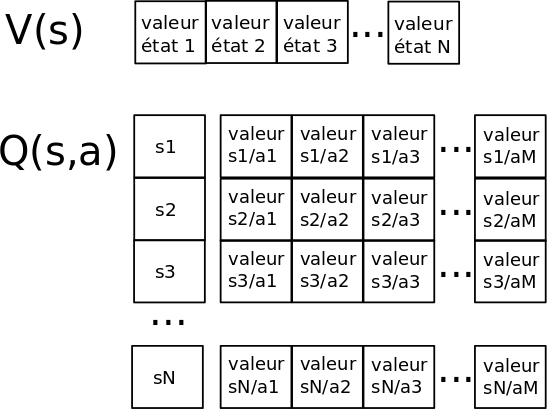
\includegraphics[scale=0.45]{ressources/v_s_vs_q_sa.png}
    \caption{Enregistrement V(s) et Q(s,a)}
    \end{figure} 
    
   \par Dans des environnements avec de nombreux (voir infinités) d'états et d'autant d'actions possibles, le stockage de la valeur de Q(s,a) devient très difficile vu la taille qu'elle représente. De plus, si l'environnement présente autant d'états et d'action possibles, l'agent va devoir effectuer beaucoup d'exploration afin d'évaluer la valeur de chaque couple (état, action), ce qui rendrait l'apprentissage extrêmement lent, voir impossible. Une solution pour palier à cet inconvénient est de remplacer le tableau Q[s][a] par un réseau neuronal. 
   
  \section{Réseaux neuronaux}
  
  \subsection{Enjeux}
  
      \par Le problème majeur des méthodes d'apprentissage par renforcement vues jusqu'ici est que lorsque l'environnement devient complexe et qu'il comporte trop d'états/actions possibles, il devient difficile (voir impossible) d'arriver à une estimation correcte que V(s) ou Q(s,a). Les réseaux neuronaux se sont révélés être de très bons estimateurs dans de nombreux champs d'applications. 
      
      \par Les réseaux de neurones sont utilisés de la manière suivante:
      
      \begin{enumerate}
      \item On crée un réseau de neurones qui a pour but d'estimer (prédire) quelque chose de précis. Au début, le réseau de neurone renvoie des réponses aléatoires. 
      \item On entraîne ce réseau de neurone en lui donnant de nombreux exemples avec la solution à estimer pour chaque exemple. (exemple d'input, solution)
      \item Au bout d'un certain nombre d'exemples donnés, le réseau de neurone s'est ajusté de sorte à pouvoir estimer (prédire) de nouveaux inputs en les estimant correctement. 
      \end{enumerate}  
      
      \par De nombreuses applications ont été trouvées pour les réseaux de neurones: on peut par exemple fournir des millier d'images comportant des tumeurs et des millier d'images ne comportant pas de tumeurs pour qu'à la fin de son apprentissage, le réseau puisse indiquer si l'image (qu'il n'a jamais vue) comporte ou ne comporte pas de tumeur. On peut également fournir un millier d'images de chiffres écrits à la main pour qu'à la fin de son apprentissage, le réseau puisse reconnaître le chiffre écrit dans une image quelconque que le réseau n'a pas encore vu. Le champ d'application est vaste: de la reconnaissance vocale à la proposition de contenu personnalisé pour Youtube ou Facebook, de nombreux domaines utilisent les réseaux neuronaux, suivant ce même principe de base. (Apprentissage, puis utilisation pour prédire quelque chose). 
      
      \par Dans le cas de l'apprentissage par renforcement, les réseaux de neurones permettent d'approximer correctement les fonctions V(s) ou Q(s,a) dans de nombreux environnements. L'utilisation d'un réseau de neurone permet les méthodes telles que le Deep Q-Learning que nous verrons dans le prochain chapitre. 
      
  \subsection{Présentation}
  
    \par Un réseau de neurones est constitué des parties suivantes: 

    \renewcommand{\labelitemi}{\textbullet}
    \begin{itemize}
    \item Une couche "d'input", représentant la couche par laquelle les données rentrent dans le réseau. Dans le cas d'images, une image est donnée à la fois. Dans le cas de l'apprentissage par renforcement, un état est donné à la fois. 
    \item Un certain nombre de couches, appelées "hidden layers". C'est dans ces couches que le réseau neuronal fait ses calculs pour effectuer une prédiction. 
    \item Une couche "d'output". C'est à travers cette couche que le résultat de la prédiction est transmise. 
    \end{itemize}    
    
    \par L'idée est que chaque neurone est relié à tous les neurones de la couche suivante, afin d'effectuer un calcul particulier à chaque couche. A la fin, la couche "output" indique le résultat de la prédiction du réseau neuronal. 
    
    \begin{figure}[!h]
    \center
    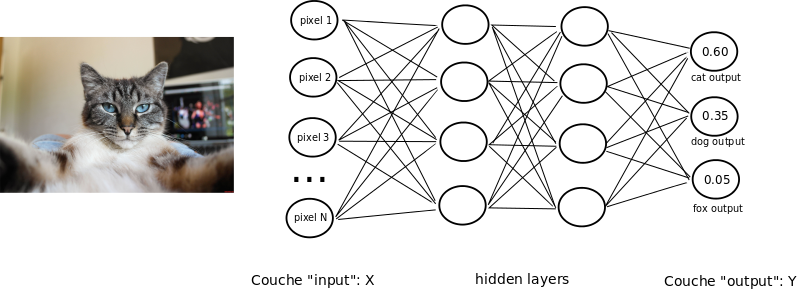
\includegraphics[scale=0.56]{ressources/nn_presentation_1.png}
    \caption{Réseau neuronal: présentation 1}
    \end{figure} 
    
    \par Dans ce premier exemple, le but du réseau neuronal est de prédire si l'image donnée dans la couche "input" est un chat, un chien, ou un renard. Le résultat de la prédiction indique que le réseau neuronal estime que l'image est à 60\% un chat, à 35\% un chien, et à 5\% un renard. Pour interpréter le résultat, on prends le neurone de sortie dont l'estimation est la plus haute: cela correspond à la sorte "chat", ce qui indique que le réseau neuronal a estimé que l'image donnée en entrée est un chat. 
    
    \begin{figure}[!h]
    \center
    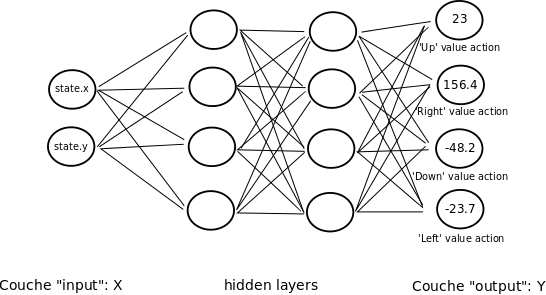
\includegraphics[scale=0.68]{ressources/nn_presentation_2.png}
    \caption{Réseau neuronal: présentation 2}
    \end{figure} 
    
    \par Dans le deuxième exemple, le but du réseau neuronal est de prédire la valeur de Q(s,a) dans l'environnement GridWorld. En input, on passe l'état dans lequel l'agent se trouve (les valeurs x et y représentant l'état). En sortie, le réseau indique l'estimation de la valeur de chaque action possible. Si l'agent ne décide pas d'effectuer une action aléatoire, l'agent prendra l'action dont la valeur est la plus haute: dans ce cas il s'agit de l'action 'Right'. 
    
  \subsection{Prédiction}

  \subsubsection{Notion de base}

    \par Pour décrire le fonctionnement d'un réseau neuronal, nous commencerons par la manière dont il effectue les prédictions. 
    
    \par Prenons l'exemple le plus simple: une valeur d'entrée (un neurone d'entrée) dont la valeur est x, une simple couche cachée d'un seul neurone contenant un poids w (weight), et une seule valeur de sortie (un seul neurone d'output) qui ne fait rien d'autre que ressortir la valeur de la couche cachée. La prédiction du neurone est calculée comme suit: 
    
    \begin{figure}[!h]
    \center
    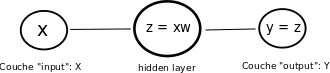
\includegraphics[scale=0.74]{ressources/nn_theory_1.png}
    \caption{Réseau neuronal: théorie 1}
    \end{figure} 
    
    \par Le but de chaque neurone caché est de prendre la valeur d'entrée, de modifier cette valeur en fonction de poids (w) (weight) que le neurone contient, et de transmettre son résultat au neurone suivant. Dans cet exemple, la prédiction vaudra: $y = z = xw$

  \subsubsection{Notation matricielle}
    
    \par Prenons maintenant le même exemple, mais avec deux valeurs en entrées. $x_1$ et $x_2$. La théorie veut que le neurone caché doit avoir 2 poids afin d'effectuer son calcul. 
    
    \begin{figure}[!h]
    \center
    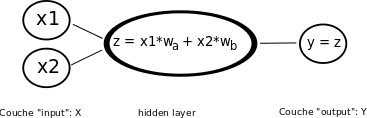
\includegraphics[scale=0.68]{ressources/nn_theory_2.png}
    \caption{Réseau neuronal: théorie 2}
    \end{figure} 
    
    \par Dans cet exemple, la prédiction vaut donc $y = z = x_1w_a + x_2w_b$
    
    \par On peut reconnaître le caractère matriciel de la prédiction et représenter la prédiction selon la notation suivante. X représente les valeurs d'entrées, W représente les poids du neurone caché, Z représente le résultat du neurone caché, et Y représente la valeur de sortie: 
    
    \begin{eqnarray}
    X &=& \begin{pmatrix} x_1 \\ x_2 \end{pmatrix} \\
    W &=&  ( w_a , w_b ) \\
    Z &=& WX  = ( w_a , w_b )\begin{pmatrix} x_1 \\ x_2 \end{pmatrix} = (x_1w_a+x_2w_b)\\
    Y &=& Z = (x_1w_a+x_2w_b)
    \end{eqnarray}
    
    \par À noter que dans la théorie qui suit, nous utiliserons la notation 'X' (majuscule) pour définir une entrée (couche input), et la notation 'Y' (majuscule) pour définir les valeurs de sortie (output). 
    
    \par Grâce à la notation matricielle, on peut maintenant imaginer un réseau avec 2 entrées et une couche de 2 neurones cachés. Comme la sortie de la couche cachée contient 2 valeurs et qu'on décide que le neurone de sortie ne fait toujours rien d'autre que de copier la sortie de la couche cachée, le neurone de sortie renverra 2 valeurs en sortie. 
    
    \begin{figure}[!h]
    \center
    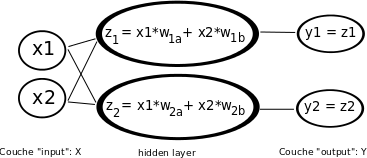
\includegraphics[scale=0.74]{ressources/nn_theory_3.png}
    \caption{Réseau neuronal: théorie 3}
    \end{figure} 
    
    \begin{eqnarray}
    X &=& \begin{pmatrix} x_1 \\ x_2 \end{pmatrix} \\
    W &=& \begin{pmatrix} w_{1a} , w_{1b} \\ w_{2a}, w_{2b} \end{pmatrix} \\
    Z &=& WX  = \begin{pmatrix} w_{1a} , w_{1b} \\ w_{2a}, w_{2b} \end{pmatrix}\begin{pmatrix} x_1 \\ x_2 \end{pmatrix} = \begin{pmatrix} w_{1a}x_1 + w_{1b}x_2 \\ w_{2a}x_1+w_{2b}x_2 \end{pmatrix} \\
    Y &=& Z = \begin{pmatrix} w_{1a}x_1 + w_{1b}x_2 \\ w_{2a}x_1+w_{2b}x_2 \end{pmatrix}
    \end{eqnarray}
    
    \par Bien entendu, si l'on souhaite n'avoir qu'une valeur en sortie, il convient de modifier le neurone de sortie de sorte à ce qu'il fasse lui aussi un calcul dont le résultat n'a qu'une matrice de 1x1. La mécanique de base reste néanmoins la même: utiliser une version matricielle pour décrire les couches et interactions entre nos neurones. De la même manière, il est possible d'ajouter plusieurs couches cachées en représentant les matrices de la bonne manière afin d'effectuer un calcul de prédiction plus complexe. 
    

  \subsubsection{Fonction d'activation}    
  
    \par Il reste encore une notion à ajouter aux réseaux neuronaux vus jusqu'ici. Les réseaux neuronaux ont été directement inspirés des vrais réseaux de neurones et de la manière dont ils fonctionnent. En termes biologiques, un neurone fait suivre une information (valeur) uniquement si le résultat de son "calcul" est supérieur à un certain seuil. En d'autres termes, un neurone ne renvoie une information que si il a suffisamment été excité. 
    
    \begin{figure}[!h]
    \center
    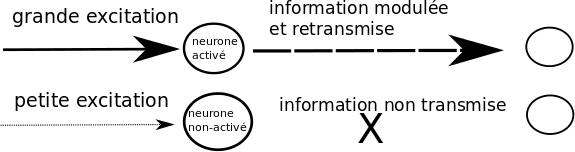
\includegraphics[scale=0.74]{ressources/nn_theory_4.png}
    \caption{Activation d'un neurone: représentation biologique}
    \end{figure} 
    
    \par Ce seuil d'activation permet aux réseaux de neurones biologiques de transmettre une information d'une manière régulée en fonction des seuils (poids) de chaque neurone. Cela permet aux réseaux de neurones biologiques d'accomplir des calculs complexes tels que la nature nous l'a montré. La notion de seuil d'excitation implique que l'intensité de chaque information transmise entre neurones doit rester comprise au sein d'un seuil biologiquement acceptable. En d'autre termes, l'intensité de l'information transmise ne peut augmenter de neurones en neurones jusqu'à atteindre une valeur trop grande, mais doit garder une intensité telle qu'un neurone puisse stopper l'information ou au contraire la retransmettre. Mathématiquement parlant, l'idée serait de garder des valeurs de sorties comprises entre [0,1]. 
    
    \par D'un point de vue complètement différent et mathématique, les opérations effectuées par les réseaux neuronaux que nous avons vues sont uniquement linéaires. Afin d'effectuer des prédictions complexes, il convient d'ajouter une notion "non-linéaire" aux opérations effectuées. Aussi, afin de pouvoir réguler facilement les poids de chaque neurone lors de la phase d'apprentissage, il convient de faire en sorte que chaque neurone renvoie une valeur de sortie comprise entre [0,1].
    
    \par Ainsi, chaque neurone passe son résultat dans une fonction non linéaire $f(x) -> [0,1]$. 
    
    \begin{figure}[!h]
    \center
    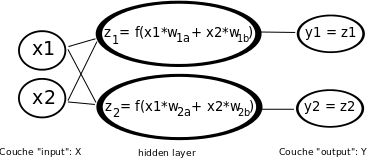
\includegraphics[scale=0.74]{ressources/nn_theory_5.png}
    \caption{Activation d'un neurone: représentation biologique}
    \end{figure} 
    
    \par L'exemple ci-dessus correspond donc à 
    
    \begin{eqnarray}
    Z &=& f(WX)  = f\left(\begin{pmatrix} w_{1a} , w_{1b} \\ w_{2a}, w_{2b} \end{pmatrix}\begin{pmatrix} x_1 \\ x_2 \end{pmatrix}\right) = f\left(\begin{pmatrix} w_{1a}x_1 + w_{1b}x_2 \\ w_{2a}x_1+w_{2b}x_2 \end{pmatrix}\right) \\
    Y &=& Z = f\left(\begin{pmatrix} w_{1a}x_1 + w_{1b}x_2 \\ w_{2a}x_1+w_{2b}x_2 \end{pmatrix}\right)
    \end{eqnarray}
    
    \par Voici les principales fonctions d'activations utilisées: 
    
    \begin{figure}[!h]
    \center
    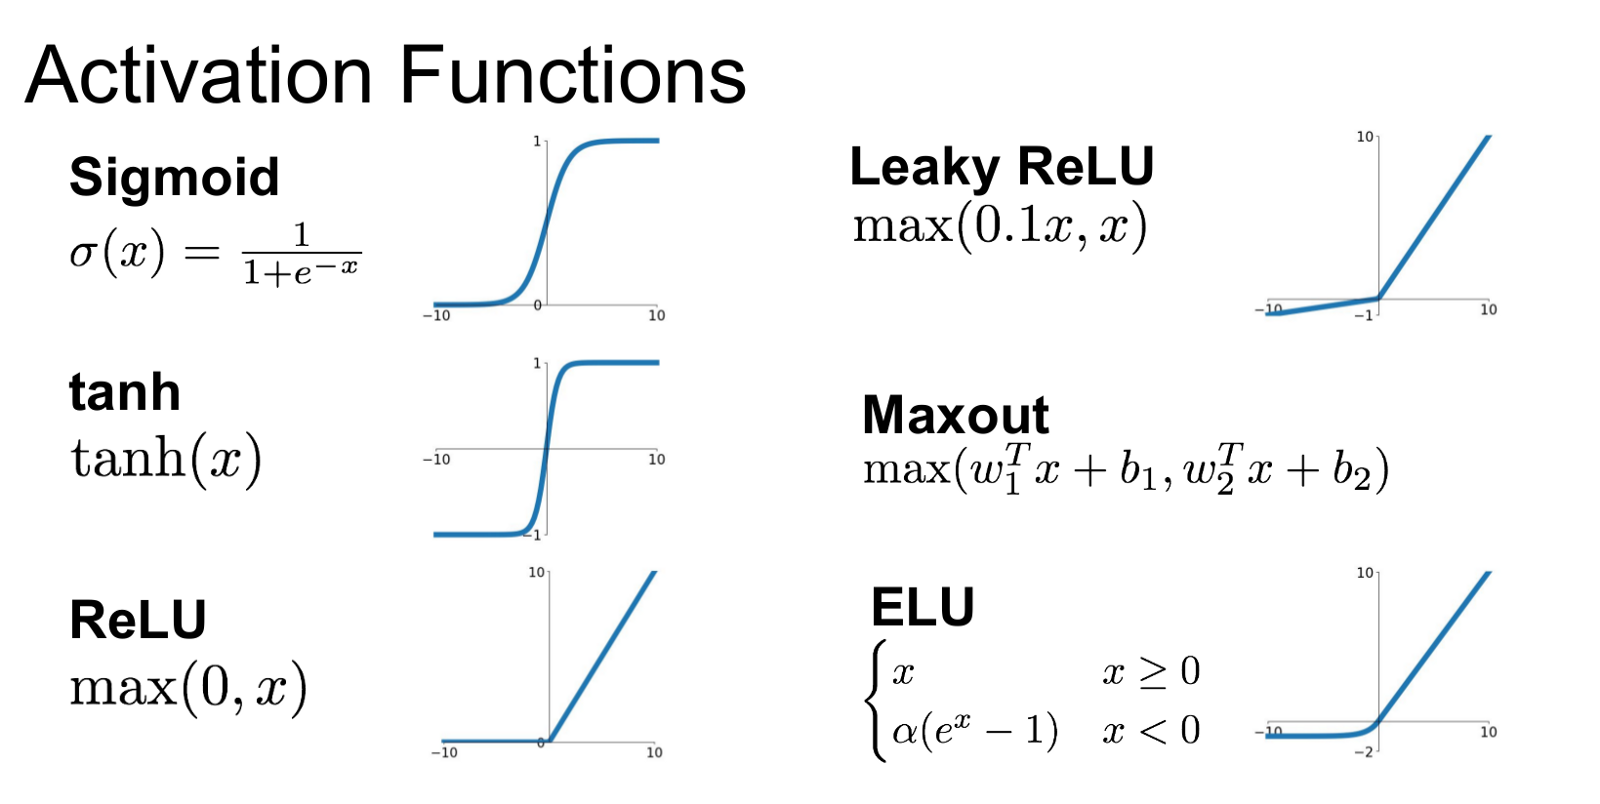
\includegraphics[scale=0.22]{ressources/activation_functions.png}
    \caption{Fonctions d'activation}
    \end{figure} 
    
    \newpage
    \par Pour terminer, le fait d'utiliser des fonctions d'activations peut comporter un problème: si un neurone émet zéro à sa sortie, il y a de fortes chances pour que le neurone suivant émette aussi 0 à sa sortie. On peut utiliser un "biais" permettant d'inhiber / stimuler l'activation d'un neurone: 
    $$Z = f(WX+b)$$
    
    \begin{figure}[!h]
    \center
    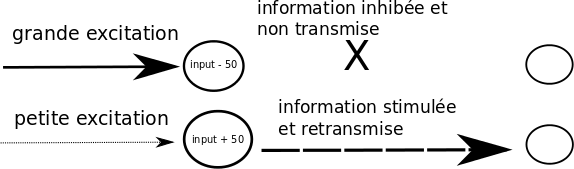
\includegraphics[scale=0.74]{ressources/nn_theory_6.png}
    \caption{Biais}
    \end{figure} 
    

    
    \par Voici donc 2 réseaux neuronaux définis mathématiquement selon toute la théorie qui a été dite: 
    
    \begin{figure}[!h]
    \center
    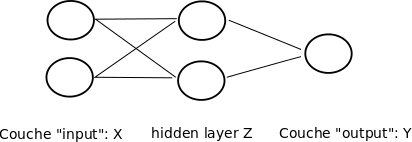
\includegraphics[scale=0.74]{ressources/nn_presentation_4.png}
    \caption{Réseau neuronal à 1 couche cachée de 2 neurones}
    \end{figure} 
    
    \begin{eqnarray}
    X &=& \begin{pmatrix} x_1 \\ x_2  \end{pmatrix}     \\
    Z &=& f\left(W_ZX+b_Z\right) = f\left(\begin{pmatrix} w_{z1a}, w_{z1b} \\ w_{z2a}, w_{z2b}\end{pmatrix}\begin{pmatrix} x_1 \\ x_2  \end{pmatrix}+\begin{pmatrix} b_{z1} \\ b_{z2}  \end{pmatrix}\right) =  \begin{pmatrix} z_1 \\ z_2  \end{pmatrix} \\
    Y &=& f_2\left( W_YZ+b_Y \right) = f_2\left( \begin{pmatrix} z_1 \\ z_2  \end{pmatrix} \begin{pmatrix} w_{ya} , w_{yb} \end{pmatrix} + b_y \right)  = (Y)
    \end{eqnarray}
    
    \newpage
    \begin{figure}[!h]
    \center
    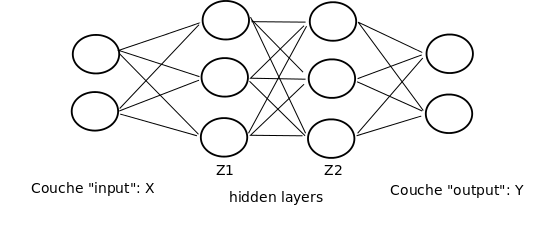
\includegraphics[scale=0.74]{ressources/nn_presentation_3.png}
    \caption{Réseau neuronal à 2 couches cachées de 3 neurones}
    \end{figure} 
    
    \begin{eqnarray}
    X &=& \begin{pmatrix} x_1 \\ x_2  \end{pmatrix}     \\
    Z1 &=& f\left(W_{z1}X+b_{z1}\right) = \begin{pmatrix} z1_{1} \\ z1_2 \\ z1_3  \end{pmatrix} \\
    Z2 &=& f_2\left(W_{z2}Z1+b_{z2}\right) = \begin{pmatrix} z2_{1} \\ z2_2 \\ z2_3  \end{pmatrix} \\
    Y &=& f_3\left( W_YZ2+b_y \right) = \begin{pmatrix} y_{1} \\ y_2  \end{pmatrix} 
    \end{eqnarray}
    

  \subsection{Apprentissage}
  
  \subsubsection{Back-propagation}
  
    \par Nous avons vu comment un neurone peut prédire un résultat Y avec des valeurs X comme entrée. Au début, tous les poids $W$ et biais $b$ de chaque neurone sont initialisés aléatoirement. Le neurone va donc prédire un résultat aléatoire. 
  
    \par L'idée de l'apprentissage est la suivante: on donne une valeur d'entrée X, dont on connaît le résultat correct de la prédiction (Target $T$). Le neurone va faire sa prédiction et sortir une valeur Y. Il faut alors ajuster chaque poids de sorte à réduire l'erreur $|Y-T|$. L'erreur peut être représentée de plusieurs manières différentes, comme par exemple $(Y - T)^2$. On représente l'erreur par une fonction $J(Y, T)$ à choix. La fonction s'appelle le "cost function". Le "phénomène" d'ajuster les poids en fonction de Y et T s'appelle Back-propagation, vu qu'un calcul va s'effectuer de la sortie vers l'intérieur du réseau de neurones. 

    \par Nous pourrions imaginer d'ajuster les poids de la manière suivante: $W = W + J(Y,T)$. Si l'erreur est grande, le poids sera "grandement" ajusté. Si l'erreur est petite, le poids sera ajusté qu'un tout petit peu. Cependant, la fonction coût $J(Y,T)$ étant positive, il faut trouver une méthode plus subtile. D'autant plus que s'il y a plusieurs couches cachées (Z1,Z2), il faudrait pouvoir ajuster les poids de Z1 uniquement en fonction de l'erreur causée par les poids de Z1, et les poids de Z2 uniquement en fonction de l'erreur causée par les poids de Z2. 

    \par La méthode utilisée pour ajuster les poids est d'utiliser la dérivée de J(Y,T). En dérivant vis à vis de chaque couche, on peut trouver l'erreur liée à chaque couche. Par conséquent, pour ajuster les poids de Z1, on effectue l'ajustement suivant: $W_{z1} = W_{z1} + \frac{dJ(Y,T)}{dW_{z1}}$. De même, pour ajuster les poids de Z2, on effectue l'ajustement suivant: $W_{z2} = W_{z2} + \frac{dJ(Y,T)}{dW_{z2}}$
  
  \subsubsection{Gradient Descent}
  
    \par Une dernière subtilité doit être ajoutée à la manière dont les poids sont ajustés. Afin d'éviter d'ajuster les poids de manière trop brutale, on ajuste (à nouveau) par une fraction $\alpha$ (learning rate). Ainsi, le méthode utilisée devient la suivante, et s'appelle la méthode du Gradient Descent: 
    
    $$W = W + \alpha \frac{dJ(Y,T)}{dW}$$
    
    \par Pour donner un exemple de calcul, prenons un cas simple, un réseau avec une couche d'entrée et une couche de sortie. (Pas de couche cachées).
    
    \begin{figure}[!h]
    \center
    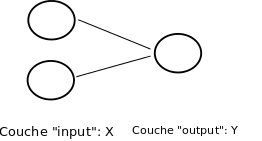
\includegraphics[scale=0.74]{ressources/nn_presentation_5.png}
    \caption{Réseau neuronal à 1 couche d'entrée et 1 couche de sortie}
    \end{figure} 
    
    \begin{eqnarray}
    Y &=& f(W_YX+b_Y) \\
    \frac{dJ}{dW_Y} &=& \frac{dJ}{dY} \frac{dY}{dW_Y} = \frac{dJ}{dY} \frac{dY}{df}\frac{df}{dW_Y}
    \end{eqnarray}
    
    \par Grâce au fait que nous travaillons avec des dérivées, l'on peut ainsi développer suffisamment pour pouvoir effectuer le calcul de $\frac{dJ}{dW_Y}$
    
    \newpage
    \par Prenons maintenant un exemple avec une couche d'entrée, une couche cachée et une couche de sortie: 
    
    \begin{figure}[!h]
    \center
    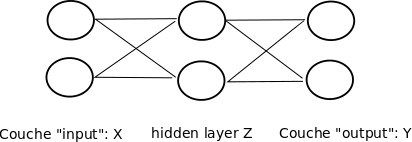
\includegraphics[scale=0.74]{ressources/nn_presentation_6.png}
    \caption{Réseau neuronal à 1 couche d'entrée, 1 couche cachée et 1 couche de sortie}
    \end{figure} 
    
    \begin{eqnarray}
    Z &=& f\left(W_ZX+b_Z\right) \\
    Y &=& f_2\left( W_YZ+b_Y \right) 
    \end{eqnarray}
    
    \par À présent, il y a deux matrices de poids à ajuster: $W_Y$ et $W_Z$. Il faut calculer leur dérivées séparément: 
    
    \begin{eqnarray}
    \frac{dJ}{dW_Y} &=& \frac{dJ}{dY} \frac{dY}{dW_Y} = \frac{dJ}{dY} \frac{dY}{df_2}\frac{df_2}{dW_Y} \\
    \frac{dJ}{dW_Z} &=& \frac{dJ}{dY} \frac{dY}{dW_Z} = \frac{dJ}{dY} \frac{dY}{df_2}\frac{df_2}{dW_Z} = \frac{dJ}{dY} \frac{dY}{df_2}\frac{df_2}{dZ}\frac{dZ}{dW_Z} = \frac{dJ}{dY} \frac{dY}{df_2}\frac{df_2}{dZ} \frac{dZ}{f_1}\frac{f_1}{dW_Z} 
    \end{eqnarray}

    \par Nous constatons (heureusement) qu'un certain schéma se répète dans le calcul des $\frac{dJ}{W_i}$, permettant ainsi le calcul des dérivées automatiquement par programmation. Plusieurs librairies fournissent cette possibilité. Pour ce travail de bachelor, la librairie TensorFlow développée par Google a été utilisée. 
    
    \par Pour conclure cette section, il est important de signaler qu'un réseau de neurone ne peut s'ajuster qu'avec un seul X et T. Il faut bien entendu répéter le calcul de back-propagation un grand nombre de fois afin d'arriver à des valeurs des poids permettant un pourcentage de prédiction correct. Une fois le réseau de neurones bien entraîné (après avoir répété la back-propagation de nombreuses fois), on peut ensuite fournir une valeur X sans connaître son résultat correct, mais en osant espérer que la prédiction sera correcte. 
  
  \section{Algorithme Deep Q-Network (DQN)}
  
    \par Dans la section "Q-Learning, nous avons vu une méthode pour enseigner à un agent comment apprendre à évoluer dans un environnement donné en explorant les actions possibles. La méthode s'avère efficace lorsque l'environnement ne possède qu'une petite quantité d'états / actions possibles. Dans ces petits environnements, l'agent peut garder une copie de chaque états et actions visitées afin d'estimer correctement la fonction Q(s,a) de sorte à apprendre à savoir quelle action effectuer pour un état donné, dans le but d'effectuer un score maximal lors d'un épisode. \\ 
   Lorsque l'environnement devient plus complexe, l'espace état / actions devient beaucoup plus grand et la tâche devient presque impossible étant donné la taille du tableau Q(s,a) à garder en mémoire, et le temps nécessaire pour explorer correctement tous les couples "état / action". Les réseaux neuronaux constituent une solution  adéquate pour effectuer une estimation complexe d'un problème donné. L'enjeu du Deep Q-learning est d'utiliser les réseaux neuronaux pour effectuer une estimation suffisante de la fonction Q(s,a) sans devoir connaître / explorer l'espace complet état / actions d'un environnement donné. Un réseau neuronal peut être appelé "Deep neural network" lorsque un réseau neuronal comprends de nombreuses couches cachées; la notion de "Deep" dans "Deep Q-learning" correspond donc à appliquer la méthode Q-learning avec un réseau de neurones à plusieurs couches cachées (hidden layers). 
   
   \par Dans le cadre de ce travail, la valeur des actions $a$ en fonction de l'état $s$ $Q(s,a)$ est définie par la prédiction d'un réseau neuronal. Nous fournissons un vecteur d'entrée X = s représentant l'état de l'environnement. Par exemple: 
   
  \begin{lstlisting}[language=python]
  X = s = [agent.x, agent.y, ennemy.x, ennemy.y]
  \end{lstlisting}
   
   \par Le résultat du réseau neuronal est une estimation de $Q(s,a)$ pour chaque action possible lors de l'état $s$. La taille du vecteur de sortie correspond au nombre total d'actions possibles lors de l'état $s$. L'action choisie sera l'index correspondant à la plus haute valeur rencontrée. 

  \begin{lstlisting}[language=python]
  Y = predicted_values = [value_action1, value_action2, value_action3, value_action4]
  action = argmax[predicted_values]
  \end{lstlisting}   
  
  \par Une action est donc un nombre entier compris entre $[0, nb\_actions\_possibles]$

  \subsection{Mise à jour de la fonction Q(s,a): ajustements à faire}
  
   \par Afin de faire fonctionner un agent avec la méthode Q-Learning utilisant un réseau neuronal pour estimer la valeur Q(s,a), il y a deux ajustements principaux à faire pour mettre à jour la fonction Q(s,a). 
  
  \subsubsection{Experience Replay}
  
  \par Comme évoqué lors du chapitre sur les réseaux neuronaux, afin qu'un réseau neuronal puisse apprendre correctement à estimer son sujet, les valeurs d'entrées X lors de la phase d'apprentissage doivent être suffisamment homogènes afin que l'apprentissage soit le plus complet possible. Or, l'idée du Q-Learning est d'ajuster Q(s,a) à chaque état parcouru de l'agent. Imaginons que l'agent commence toujours un épisode dans un même état initial: \\
  Si l'agent met à jour son réseau neuronal (Q(s,a)) à chaque état qu'il rencontre, l'apprentissage de Q(s,a) sera biaisé dans le sens où il va renforcer l'ajustement de Q(s,a) sur les premiers états (récurrents à chaque nouvel épisode), et laissera les états suivants (sporadiques) de coté pour son apprentissage. Il en résultera par exemple que l'agent connaisse les 20 premières actions à faire, mais sera incapable d'estimer correctement la suite des actions à faire. 
  
  \par Pour palier à ceci, l'idée est d'enregistrer tous les états / actions / récompenses dans une liste d'échantillons dont la longueur est définie par le programmeur. D'ici à ce que la liste d'échantillons ne soit pas pleine, l'agent ne met pas à jour la fonction Q(s,a). Si la liste est pleine, les échantillons (états / actions / récompenses) les plus vieux sont remplacés par les nouveaux échantillons rencontrés. 
  
  \par Une fois que l'on dispose d'une liste d'échantillons suffisamment grande, l'agent met à jour la fonction Q(s,a) en choisissant \textbf{aléatoirement} une \textbf{petite} partie de ces échantillons (batch). L'on par exemple mettre à jour la fonction Q(s,a) à chaque nouvel épisode, pour autant que la liste soit suffisamment grande afin de permettre de choisir \textbf{aléatoirement} un groupe d'échantillons de la liste d'échantillons. L'on peut ainsi supposer que l'agent puisse mettre à jour la fonction Q(s,a) parmi un choix d'échantillons aléatoires et suffisamment homogène. 
  
  \subsubsection{Apprentissage du réseau neuronal: Estimation Y et Target T}
  
    \par L'autre inconvénient majeur d'utiliser un réseau neuronal est que pour l’entraîner, il nous faut d'entrées X et connaître les solutions T pour chaque entrée X. En effet, le réseau neuronal ajuste ses poids lors de l'apprentissage à l'aide de la fonction J(Y, T). Or, nous ne connaissons pas T étant donné que l'idée du Q-Learning est d'explorer sans connaître son environnement. Comment choisir T étant donné que la meilleure estimation de Q(s,a) est définie par la prédiction de Q(s,a) par QNetwork? 
    
    \par En d'autres termes, si nous utilisons pour chaque X, une solution T = Y, le taux d'erreur sera de 0 et l'agent n'apprendra rien: le réseau neuronal QNetwork n'apprendra rien étant donné que la solution T correspond à la prédiction Y. 
    
    \par Une méthode qui a fait (bizarrement) ses preuves et d'avoir deux réseaux neuronaux. Le réseau pour estimer Q(s,a) (QNetwork), et un deuxième réseau pour estimer les solutions T (TNetwork). TNetwork est une copie conforme à QNetwork, à la seule différence est que TNetwork est copié de QNetwork toutes les N actions de l'agent. À l'action "0" de l'agent, QNetwork et TNetwork sont exactement les mêmes et l'apprentissage de Q(s,a) ne se fera pas. En revanche, pour les actions suivantes, QNetwork sera mis à jour et TNetwork reste le même, continuant à prédire ses valeurs T. \\
    Ainsi, Q(s,a) pourra être mise à jour étant donné que les valeurs Q(s,a) = Y de QNetwork(s) et les valeurs de TNetwork(s) = T ne fournirons pas les mêmes valeurs. 
    
    \par Bien entendu, toutes les N actions, le réseau TNetwork sera à nouveau copié depuis QNetwork car QNetwork tends à s'ajuster correctement. Dans l'implémentation du dernier exercice du rapport, TNetwork est copié depuis QNetwork toutes les 100 actions (hyper-paramètre COPY\_TARGET\_PERIOD). 
    
   \subsection{Pseudo-code de l'algorithme Deep Q-Network} 
   
   \subsubsection{Partie principale}
   
   \par Voici un pseudo code effectuant l'algorithme Deep Q-Network: 
   
   \begin{lstlisting}[language=python]
#*****
#MAIN
#*****
# phase d'apprentissage
world = new World()
max_episodes = 100000
gamma = 0.9
epsilon = 0.1
alpha = 0.1
QNetwork = NeuralNetwork()
TNetwork = NeuralNetwork(QNetwork)
experience = []
min_experience_size = 10000
cp_target_period = 10000
batch_size = 32
  
for i in range(max_episodes):
  state = world.reset()
  while not world.game_over():
    action = choose_action(state, epsilon, QNetwork)
    reward, next_state = world.do_action(state, action)

    experience.append((state, next_state, action, reward, game_over)) 
    if experience.length >= min_experience_size:
      train(QNetwork, TNetwork, experience, batch_size, alpha)

    if i % cp_target_period == 0:
      TNetwork.copy_from(QNetwork)
        
    state = next_state
    
        
# phase une fois l'apprentissage effectué
state = world.reset()
while not world.game_over():
  action = choose_action(state, epsilon, QNetwork)
  state, _ = world.do_action(action)
        
  \end{lstlisting} 

   \subsubsection{Fonction choose\_action()}

   \par Voici le pseudo code de la fonction choose\_action():  
  
  \begin{lstlisting}[language=python]
  
def choose_action(state, epsilon, QNetwork):
  if random() < epsilon:
    action = random_action()
  else:
    prediction = QNetwork.predict(state)
    action = argmax(prediction)
 return action
 
  \end{lstlisting} 
  
  \par Un état est représenté par un vecteur contenant les informations suffisantes pour illustrer l'état du jeu.
  \begin{lstlisting}[language=python]
  state = [agent.x, agent.y, ennemy.x, ennemy.y]
  \end{lstlisting} 
  
  \par La prédiction du réseau QNetwork prend en entrée le vecteur state, et retourne en sortie un vecteur contenant les récompenses (rewards) estimées pour chacune des actions possibles. La taille du vecteur de sortie correspond donc au nombre d'actions possibles pour l'agent. 
  
  \begin{lstlisting}[language=python]
  prediction = [ra_1, ra_2, ra_3, ra_4, ra_5] = QNetwork.predict(state)
  \end{lstlisting} 
  
  \par La fonction choose\_action() retourne l'index de la plus grande récompense estimée. Dans ce travail de bachelor, cet index équivaut à l'action choisie. Par exemple: 
  
 \begin{lstlisting}[language=python]
  prediction = [1.5, 12, -2, 1.4, 0.56] = QNetwork.predict(state)
  action = 1 = argmax(prediction)
  \end{lstlisting}
  
   \subsubsection{Fonction train()}
     
  \begin{lstlisting}[language=python]
  
def train(QNetwork, TNetwork, experience, batch_size, alpha):
  inputs = []
  choosen_actions = []
  targets = []
 
  batch = experience.pop_batch(batch_size)
  for sample in batch:
    s1, s2, w, game_over, action = sample.extract()

    inputs.append(s1)
    
    predicted_values = QNetwork.predict(s1)
    predicted_values = 0 for all values except for predicted_values[action]
    choosen_actions.append(predicted_values)
    
    target_Q_values_s2 = TNetwork.predict(s2)
    action_value = target_Q_values_s2[action]
    target = zeros(nb_posible_actions)
    target[action] = r if game_over else r + gamma * action_value
    targets.append(target)
    
  QNetwork.back_propagation(inputs, choosen_actions, targets, alpha)
    \end{lstlisting} 
  
  \par Pour entraîner le réseau QNetwork, celui-ci a besoin d'un input (vecteur représentant l'état de l'environnement), d'un vecteur représentant les valeurs qu'il a estimées (action), et les valeurs correctes qu'il aurait retourner. 
  
  \begin{lstlisting}[language=python]
  state = [agent.x, agent.y, ennemy.x, ennemy.y]
  predicted_values = [1.5, 12, -2, 1.4, 0.56]
  correct_values = target =  [2.1, 6, -2.1, 3.5, 2.21]
  \end{lstlisting} 
  
  \par Les valeurs correctes ne sont connues uniquement pour les actions qui ont été effectuées. (Pour chaque action effectuée, nous connaissons leurs récompenses et les états résultant des actions choisies. Pour chaque état, nous ne connaissons donc uniquement la valeur correcte correspondant à l'action choisie. La valeur correcte $Q(s_{visité}, a_{choisie})$ est calculée selon l'algorithme Q-Learning, en utilisant le réseau TNetwork:
  
  \begin{lstlisting}[language=python]
  target_Q_values_s2 = TNetwork.predict(s2)
  action_value = target_Q_values_s2[action]
  correct_value = target = r if game_over else r + gamma * action_value
  \end{lstlisting}   
  
  \par Or, un réseau neuronal a besoin pour s’entraîner (back-propagation) de vecteurs de la même taille que les vecteurs qu'il a en sortie. Pour entraîner le réseau uniquement sur l'action effectuée, nous créons le vecteur T (target) composé uniquement de zéros, sauf là où le réseau doit être ajusté. De même, le vecteur predicted\_values est mis à zéro partout sauf là où l'action a été effectuée. Dans cet exemple, l'action effectuée est l'action = 2. 
  
  \begin{lstlisting}[language=python]
  # avant modification
  state = [agent.x, agent.y, ennemy.x, ennemy.y] = X
  predicted_values = [1.5, 12, -2, 1.4, 0.56] = Y
  correct_values = target =  [2.1, 6, -2.1, 3.5, 2.21] = T
  
  # après modification
  state = [agent.x, agent.y, ennemy.x, ennemy.y] = X
  predicted_values = [0, 0, 0, 1.4, 0] = Y
  correct_values = target =  [0, 0, 0, 3.5, 0] = T
  \end{lstlisting} 
  
  \par De cette manière, lors du "back-propagation", l'ajustement des poids du QNetwork ne sera mis à jour que là où la dérivée $\frac{dJ(Y,T)}{dW} \neq 0$. Y = predicted\_values, et T = target.
  
  $$W = W + \alpha \frac{dJ(Y,T)}{dW}$$
  
  \par Enfin, les librairies permettent d’entraîner un réseau neuronal en lui fournissant une matrice d'inputs (X), predicted\_values (Y) et target (T) (à la place d'un vecteur à la fois). Le principe reste le même, mais cela permet d'effectuer les calculs beaucoup plus rapidement qu'en fournissant à chaque fois qu'un seul vecteur. C'est la raison pour laquelle le pseudo code entraîne le QNetwork avec des matrices (X = inputs), (Y = predicted\_values) et (T = targets). 
  
  \chapter{Implémentation}
  
  \section{Fonctionnement}
  
  \subsection{Vue d'ensemble: choix d'une action}
  
  \par Les actions possibles dans l'environnement implémenté sont d'avancer dans une direction des points cardinaux (N, NE, E, SE, S, SO, O, NE), ou ne rien faire. Le nombre d'actions possibles équivaut donc à neuf. 

  \par Comme indiqué dans l'introduction, l'apprentissage est divisé en trois parties. Dans un premier temps, l'agent doit pouvoir évoluer dans un monde qu'avec des ennemis, en utilisant un réseau neuronal dédié estimant la meilleure action à effectuer. Dans un deuxième temps, l'agent doit pouvoir évoluer uniquement avec de la nourriture utilisant un autre réseau neuronal dédié à attraper la nourriture. Enfin, l'agent doit pouvoir évoluer dans un monde "complet", avec ennemis et nourriture. Dans ce dernier cas, l'agent dispose de trois réseaux neuronaux: un pour choisir la meilleure action de sorte à éviter les ennemis, un deuxième estimant la meilleure action pour attraper la nourriture, et un troisième réseau neuronal estimant quel est le meilleur réseau neuronal à écouter: effectuer l'action évitant les ennemis, ou effectuer l'action pour attraper la nourriture. 
  
   \begin{figure}[!h]
   \center
   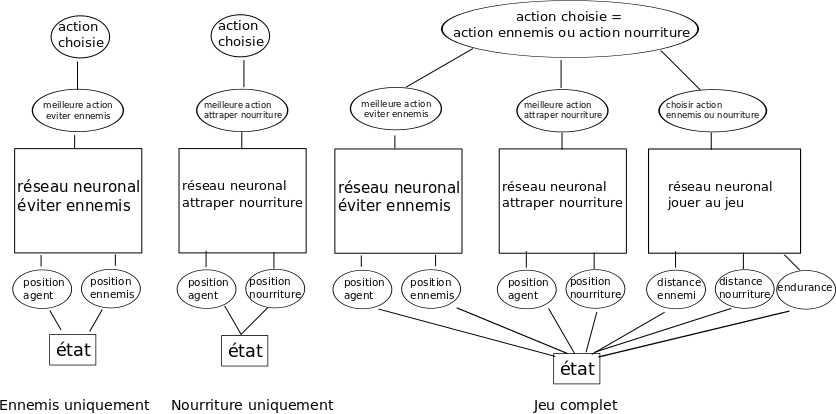
\includegraphics[scale=0.6]{ressources/vue_ensemble_reseaux_agents.png}
   \caption{Vue d'ensemble: choix d'une action}
   \end{figure} 
  
  \par Il aurait été possible de n'utiliser qu'un grand réseau neuronal pour apprendre directement à jouer dans un monde complet, sans fractionner l'apprentissage. Il y a plusieurs raisons pour laquelle nous avons choisi d'utiliser plusieurs réseaux neuronaux: la première vient de la difficulté à choisir une fonction de récompense adéquate à ce que nous voulons apprendre à l'agent. L'apprentissage est plus efficace lorsque la fonction de récompense renforce le comportement de l'agent dans un contexte bien spécifique (éviter ennemis ou attraper la nourriture). \\
  La deuxième raison vient du fait que plus un réseau neuronal est grand, moins l'apprentissage est rapide. Plus il y a d'inputs dans le réseau neuronal, plus ce dernier est grand. Il est donc préférable d’entraîner l'agent sur des problèmes spécifiques avant de l’entraîner à jouer de manière complète. Comme indiqué dans la figure ci-dessus, avec cette méthode, le réseau neuronal capable de jouer pas besoin de beaucoup d'inputs. Ce dernier ne connaît même pas la position de la nourriture, de l'agent ni des ennemis. \\
  Enfin, une fois qu'un agent a appris une tâche spécifique, il n'y a pas besoin de le ré-entraîner  (pour autant que le monde et les inputs concernés ne changent pas). Imaginons maintenant que nous ayons utilisé un seul grand réseau neuronal pour jouer, et que l'on veuille ajouter une nouvelle tâche à apprendre à l'agent. Il faudrait ré-entraîner le tout depuis zéro. En fractionnant l'apprentissage en tâches spécifiques, il y aurait seulement besoin d’entraîner le nouveau réseau concernant la nouvelle tâche, et le réseau capable de jouer.  
  
  \subsection{Apprentissage}
    
  \par L'apprentissage de l'agent se fait à travers trois scripts qui durent entre 24 et 72 heures. Chaque script a pour but d'enseigner à l'agent une "capacité": éviter les ennemis, attraper la nourriture ou apprendre à jongler entre les deux pour jouer au jeu complet. Chaque capacité est contenue dans un réseau neuronal QNetwork; l'apprentissage correspond à modifier les poids de ces réseaux (back-propagation) de sorte à pouvoir estimer correctement la fonction $Q(s,a)$.

  \renewcommand{\labelitemi}{\textbullet}
  \begin{itemize}
  \item \textbf{trainer\_avoid\_ennemies.py}: 
      \begin{enumerate}
      \item charger un monde qu'avec des ennemis
      \item créer un nouveau réseau neuronal 
      \item entraîner l'agent à éviter les ennemis
      \item enregistrer l'état du réseau neuronal lorsque l'agent  a appris à éviter les ennemis puis quitter le script
      \end{enumerate}
  \item \textbf{trainer\_fetch\_object.py}: 
      \begin{enumerate}
      \item charger un monde qu'avec de la nourriture
      \item créer un nouveau réseau neuronal
      \item entraîner l'agent à attraper la nourriture
      \item enregistrer l'état du réseau neuronal lorsque l'agent  a appris à attraper la nourriture puis quitter le script
      \end{enumerate}  
  \item \textbf{trainer\_play\_game.py}:
      \begin{enumerate}
      \item charger le monde complet (ennemis + nourriture)
      \item charger les deux réseaux neuronaux estimant correctement les actions pour éviter les ennemis et attraper la nourriture
      \item créer un nouveau réseau neuronal (qui apprendra à jongler entre les deux réseaux neuronaux chargés)
      \item entraîner l'agent à jouer au jeu complet
      \item enregistrer l'état du réseau neuronal lorsque l'agent  a appris à jouer au jeu complet puis quitter le script
      \end{enumerate}
  \end{itemize}
  
  \subsection{Regarder l'agent jouer}
  
  \par Trois scripts supplémentaires ont été créés permettant de visualiser en temps réel l'agent évoluer dans le monde voulu. Ces scripts chargent le mondent, chargent l'agent en important les réseaux neuronaux adéquats à partir des sauvegardes contenues dans le dossier \textit{saves}. 

  \renewcommand{\labelitemi}{\textbullet}
  \begin{itemize}
  \item \textbf{see\_avoid\_ennemies\_in\_action.py}
  \item \textbf{see\_fetch\_object\_in\_action.py}
  \item \textbf{see\_play\_game\_in\_action.py}
  \end{itemize}
  
  \subsection{Tester soi-même l'environnement}
  
  \par Afin de tester le monde dans lequel va évoluer l'agent, il est possible d’exécuter le fichier \textbf{World.py} afin de pouvoir jouer soi-même. 
  
  \begin{lstlisting}[language=bash]
  $ python world.py
  \end{lstlisting} 
  
  \subsection{Configuration}
  
  \par Le choix de tous les hyper-paramètres tels que la fonction de récompense, le discount factor $\gamma$, la taille de l’expérience, le learning rate $\alpha$, etc. sont tous définis dans les scripts directement (et null part ailleurs). Cela facilite grandement lorsque qu'il s'agit de voir quels hyper-paramètres ont été utilisés lorsque un agent a spécialement réussi un apprentissage. De plus, à chaque fois que l'un script de type \textit{trainer} est executé, une copie de celui-ci est enregistrée dans le dossier choisi pour les sauvegardes. 
  
  \par Dans cette sous-section, nous passons en revue le contenu des scripts définis plus haut. 
  
  \subsubsection{Chargement de l'environnement}
  
  \par Le chargement de l'environnement se fait de la manière suivante en choisissant la configuration désirée. La fonction de récompense est définie à ce moment là: c'est elle qui retourne la récompense. Cette fonction est appelée par le monde (classe World) lorsque l'agent effectue une action dans celui-ci. A noter que pour les scripts de type \textbf{see\_*\_in\_action.py}, la fonction récompense n'est pas utilisée étant donné que l'agent n'est pas chargé pour apprendre. L'exemple suivant est importé du script \textbf{trainer\_fetch\_object.py}.
  
  \begin{lstlisting}[language=python]
# create the world
def reward_function(world):
    if world.game_over:
        return - 5
    max_distance = 73
    return (1 - Direction.distance(world.agent, world.food) / max_distance)
world_config = {
    'food' : True,
    'ennemies': False,
    'print_reward' : False,
    'reward_function': reward_function
}
world = World(world_config)
world.reset()
  \end{lstlisting}   
  
  \subsubsection{Choix du dossier de sauvegarde et création de graphiques Tensorboard}
  
  \par Les réseaux neuronaux sont une boite noire difficiles à déboguer. Afin de visualiser l'apprentissage par des graphiques, nous utilisons l'outil \textit{Tensorboard} disponible dans la librairie \textit{Tensorflow}. La création des graphiques et le choix du dossier dans lequel vont être enregistrés les réseaux neuronaux se définissent de la manière suivante, à travers la classe statique \textbf{Debug}: 
  
  \begin{lstlisting}[language=python]
Debug.USE_TENSORBOARD = True
Debug.SAVE_MAIN_FILE = True
Debug.SAVE_FOLDER = '../tmp_saves/avoid_ennemies'
Debug.OUTPUT_TO_TENSORBOARD_EVERY_N_EPISODES = 5000
  \end{lstlisting}   
  
 \subsubsection{Création d'un réseau neuronal} 
 
 \par Comme vu dans la figure 3.1, un réseau neuronal doit pouvoir être configuré de sorte à ce que les entrées et sorties puissent être définies manuellement au cas par cas. Au lieu de donner l'état du monde tel quel en entrée, nous passons par une fonction \textit{input\_adapter()} qui retourne le vecteur X désiré. De même, l'on peut définir une fonction \textit{output\_adapter()} afin de convertir la sortie d'un réseau neuronal en une action particulière. La fonction \textit{output\_adapter()} est facultative. 
 
  \begin{figure}[!h]
  \center
  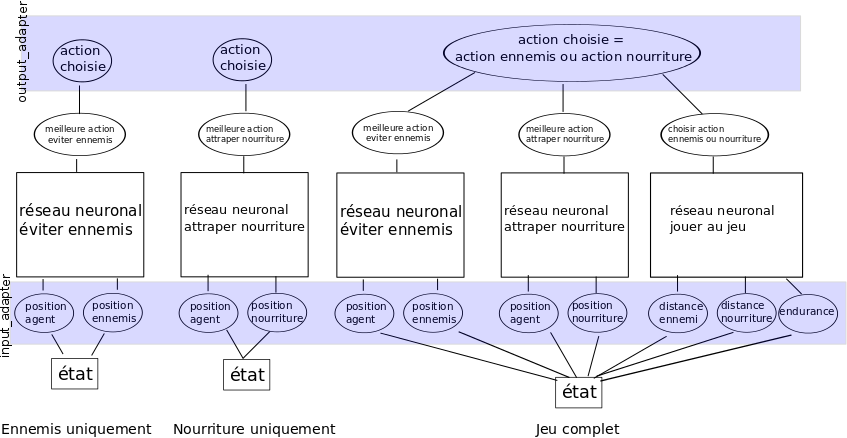
\includegraphics[scale=0.6]{ressources/input_output_adapters.png}
  \caption{Input et Output adapters}
  \end{figure} 

  \par La création d'un réseau neuronal se crée de la manière suivante. On crée d'abord un modèle contenant l'architecture du réseau neuronal, le nom de celui-ci ainsi que le learning\_rate $\alpha$. 
  
 \begin{lstlisting}[language=python]
fetch_object_model = Model (session , name, nb_input, learning_rate,
  [[size_layer1 , activation_function_layer1],
  [size_layer2 , activation_function_layer2],
  [ size_output_layer , activation_function_layer3]]
)
  \end{lstlisting}  
  
  \par Puis on crée le réseau neuronal à partir de l'architecture définie plus haut. Voici un exemple tiré du script \textbf{trainer\_fetch\_object.py}. La variable \textit{bus} contiendra les états \textit{s1} et \textit{s2} nécessaires pour définir la fonction \textit{input\_adapter}
  
  \begin{lstlisting}[language=python]
# create the neural network that will learn to fetch
fetch_object_model = Model(session, 'fetch_object', 4, 1e-1,
        [[40, 'relu'],
         [40, 'relu'],
        [Action.NB_POSSIBLE_MOVE_ACTION, 'linear']]
)
# fetch_object_model = ImportModel(session, Debug.SAVE_FOLDER, 'fetch_object')
def fetch_object_input_adapter(bus, next_state=False):
    index = 'next_state' if next_state else 'state'
    agent_position = bus[index].get_agent_position_layer()
    food_position = bus[index].get_food_position_layer()
    return [np.array([agent_position, food_position]).flatten()]

fetch_object_network = Network(
    fetch_object_model,
    fetch_object_input_adapter,
    True, # continue_exploration
    True, # is_training (has to be trained during process)
    None, # add experience hook
    None # output_adapter
)
  \end{lstlisting}  
  
  \subsubsection{Création de l'agent} 
  
  \par Maintenant que le monde et un réseau neuronal est créé, l'on peut créer l'agent. Nous définissons le reste des hyper-paramètres tels que la fonction epsilon $\epsilon$, la taille d'un batch, ou du discount factor $\gamma$. Comme il peut y avoir plusieurs réseaux neuronaux, il faut définir quel est le réseau neuronal de sortie. Dans cet exemple, la valeur epsilon $\epsilon$ reste stable durant tout l’entraînement. 

  \begin{lstlisting}[language=python]
# create agent and his hyperparameters (config)
epsilon = Epsilon(0.1)
def update_epsilon(epsilon):
    epsilon.value = epsilon.value
epsilon.set_epsilon_function(update_epsilon)

agent_config = {}
agent_config['epsilon'] = epsilon
agent_config['networks'] = [fetch_object_network]
agent_config['output_network'] = fetch_object_network
agent_config['copy_target_period'] = 10000
agent_config['min_experience_size'] = 50000
agent_config['max_experience_size'] = 400000
agent_config['batch_size'] = 32
agent_config['gamma'] = 0.5

agent = Agent(agent_config)
  \end{lstlisting} 


  \section{Architecture}
  
  \subsection{Diagramme de classes}
  
  \par Nous avons vu jusqu'ici le contenu des scripts permettant l'apprentissage de l'agent, et des scripts permettant la visualisation de l'agent en train d'évoluer dans le monde. Voici un diagramme des classes simplifié des classes utilisées par ces scripts. 
  
  \begin{figure}[!h]
  \center
  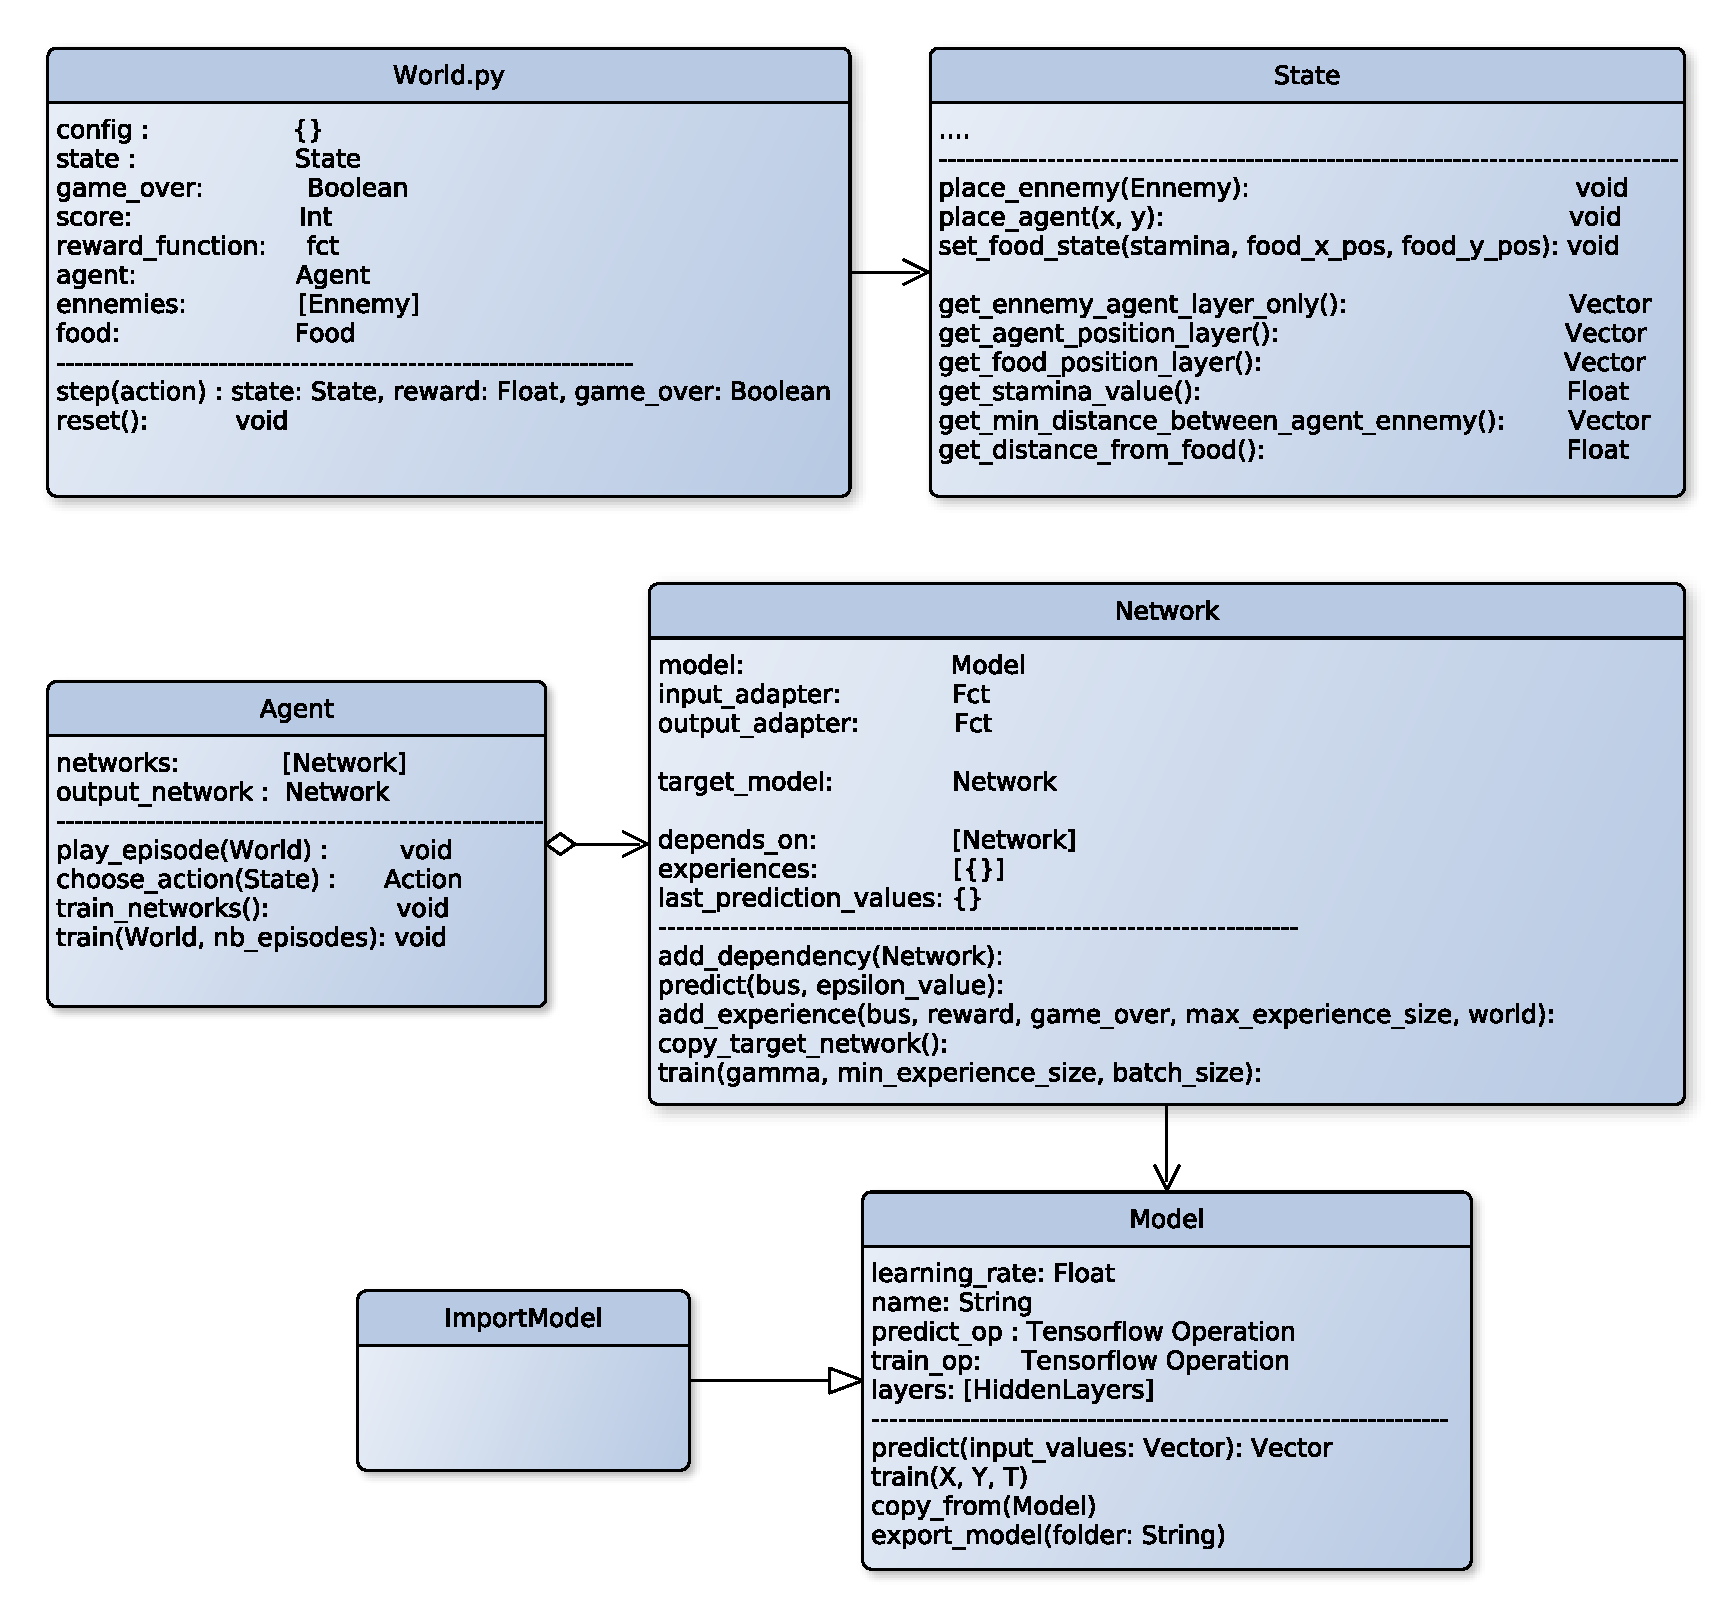
\includegraphics[scale=0.6]{ressources/class_diagram.eps}
  \caption{Diagramme des classes}
  \end{figure} 
  
  \subsection{Méthodes clés}
  
  \subsubsection{Apprentissage}
  
  \par L'apprentissage de l'agent se fait à travers sa méthode \textit{Agent.train()}, et est résumée par ceci: 
  
  \begin{lstlisting}[language=python]
def train(self, world, nb_episodes):
   for i in range(nb_episodes):
      self.play_episode(world)
  \end{lstlisting} 
  
  \par La méthode \textit{Agent.play\_episode()} est quant à elle résumée par ceci: 
  
  \begin{lstlisting}[language=python]
def play_episode(self, world, max_episode_steps=None):
  current_state = world.reset()

  episode_done = False
  while not episode_done:
      action = self.choose_action(current_state)
      next_state, reward, game_over, world_debug = world.step(action)

      if self.nb_steps_played % self.copy_target_period == 0:
         self.copy_target_networks()

      self.add_experience(next_state, reward, game_over, world)
      self.train_networks()

      if game_over: 
          episode_done = True

      current_state = next_state
      self.epsilon.update_epsilon()
      self.nb_steps_played += 1

  \end{lstlisting} 
  
  \subsubsection{Choix d'une action}
  
  \par Comme un agent peut contenir plusieurs réseaux neuronaux, il convient de choisir correctement comment choisir son action. En effet, un réseau neuronal tel que le réseau \textit{play\_game}, dépend des réseaux neuronaux \textit{avoid\_ennemies} et \textit{fetch\_object} (nourriture) avant d'indiquer l'action à effectuer. La méthode \textit{Agent.choose\_action()} est implémentée de la sorte: 
  
  \begin{lstlisting}[language=python]
def choose_action(self, state):
  self.bus['state'] = state

  nb_networks_that_predicted = 0
  while nb_networks_that_predicted != len(self.networks):
    for network in self.networks:
      if len(network.depends_on) is 0 \\
      or all(dependency.prediction_done for dependency in network.depends_on):
        network.predict(self.bus, self.epsilon.value)
        nb_networks_that_predicted += 1

  return self.output_network.get_last_action()
  \end{lstlisting} 
  

  \chapter{Résultats}
  
  \par Concevoir et implémenter l'architecture est une chose, faire en sorte que l'agent puisse apprendre correctement en est une autre. Il a beaucoup d'hyper-paramètres  à régler pour obtenir un résultat convenable. Au début du travail, il fallait faire tourner l'agent jusqu'à 14 jours avant de pouvoir affirmer si l'apprentissage se faisait ou non. De plus, étant donné qu'il y a une part de hasard dans l'apprentissage (valeurs initiales des poids $W$ des réseaux neuronaux, position des ennemis et fonction $epsilon$, l'apprentissage de l'agent peut varier d'une session à l'autre, même en gardant les mêmes hyper-paramètres. 
  
  \par Après de nombreux essais et de tests, nous présentons dans ce chapitre les paramètres principaux ayant majoritairement contribué à ce que l'agent puisse apprendre à évoluer correctement dans son environnement. 
  
  \section{Fonction récompense}
  
  \subsection{Problème rencontré}
  
  \par Un premier paramètre déterminant est le choix de la fonction récompense. Au début, afin d’entraîner l'agent à éviter les ennemis, la fonction récompense était définit comme suit: 
  
  \begin{lstlisting}[language=python]
def reward_function(world):
  if world.game_over:
    return - 1
  else:
    return 1
  \end{lstlisting} 
  
  \par L'idée est simplement de récompenser d'un point à chaque fois que l'agent effectue une action sans tomber sur un ennemi. S'il tombe sur un ennemi, l'agent reçoit un malus de 1.
  
  \par En constatant que l'apprentissage ne se faisait pas, (que le score de l'agent dans le jeu était constamment médiocre), nous avons utilisé Tensorboard afin de tracer l'histogramme des actions effectuées par l'agent, et l'histogramme de l'évolution des poids des réseaux neuronaux. 
  
  \begin{figure}[!h]
   \center
   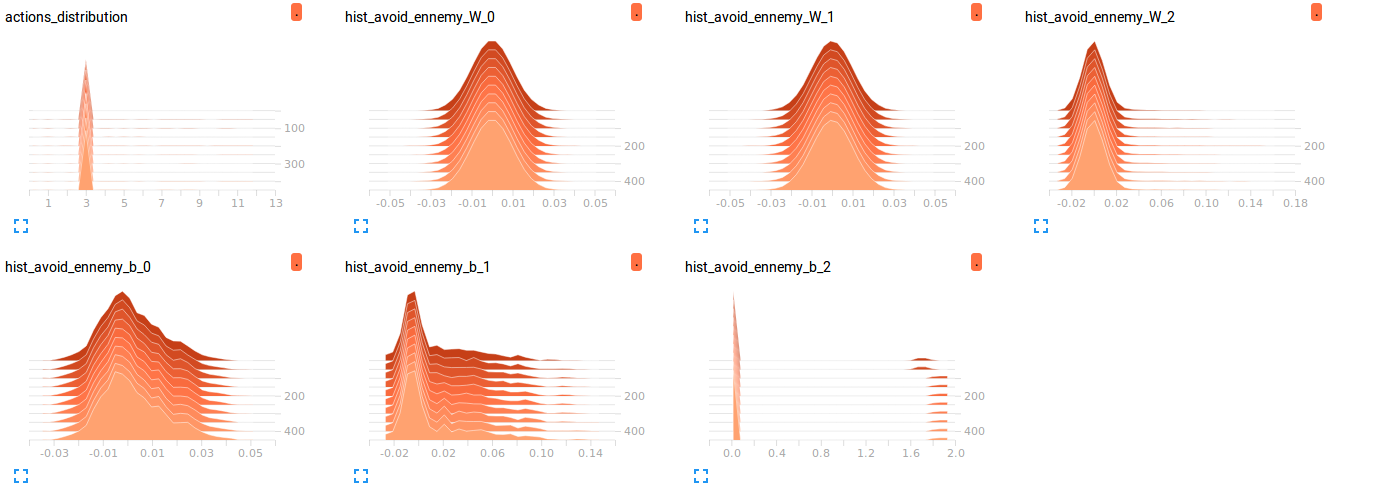
\includegraphics[scale=0.4]{ressources/bad_reward_histograms.png}
   \caption{Histogrammes des actions et poids avec une mauvaise fonction récompense}
   \end{figure} 
   
 \par Nous avons pu en déduire que l'agent n'effectuait qu'une seule action (graphique en haut à gauche), et que l'apprentissage ne se faisait pas car l'histogramme des poids (autres graphiques) n'évoluaient pas. 
  
  \subsection{Explication}
  
  \subsubsection{Début de l'agent}
  
  \par A sa création, le réseau neuronal possède des poids d'une valeur répartie aléatoirement entre $[-0.5,0.5]$. Prenons par exemple un réseau estimant la valeur $Q(s,a)$ avec une couche de sortie d'un vecteur de taille 3; c'est à dire que le réseau estime $Q(s,a)$ dans un environnement supposé où il y a 3 actions possibles. L'évaluation de la fonction $Q(s,a)$ commencera par une certaine valeur: 
  $$Q(s_t, a) = [0.1, 0.56, 0.22]$$
  
  \par À noter que l'utilisation du réseau neuronal a l'avantage de pouvoir estimer directement les 3 actions possibles, et n'a donc besoin que de l'état $t$ pour effectuer son estimation. Ainsi, au lieu de faire 3 fois le calcul $Q(s_t,a_1) = 0.1$, $Q(s_t,a_2) = 0.56$, $Q(s_t,a_3) = 0.22$, le réseau neuronal estime simplement $Q(s) = [0.1, 0.56, 0.22]$. Nous garderons cependant la notation suivante: 
  $$Q(s_t, a) = [0.1, 0.56, 0.22]$$
  
  \par Dans ce même exemple, nous prendrons la fonction récompense suivante: 
  
  \begin{lstlisting}[language=python]
def reward_function(world):
  if world.game_over:
    return - 0.5
  else:
    return 1
  \end{lstlisting} 
  
  \par En continuant l'exemple donné, l'agent choisira donc l'action numéro 2, étant donné qu'il s'agit de l'action dont la valeur est la plus haute ($0.56$). En prenant la fonction récompense vue plus haut, l'agent reçoit la récompense de $1$ pour son action numéro 2. Il stocke donc dans son expérience les valeurs suivantes: 
  
  \begin{lstlisting}[language=python]
   experience = [{'state': s_t, 'action': 2, 'reward': 1}]
  \end{lstlisting}
  
  \par Dans les états qui suivent, étant donné que le réseau neuronal est à peine créé, il y a de fortes chances qu'il donne des valeurs équivalentes à l'état $s_{t+1}$: 
  $$Q(s_{t+1}, a) = [0.101, 0.562, 0.219]$$
  
  
  \par Par conséquent, l'agent va à nouveau choisir l'action numéro 2 à l'état $s_{t+1}$. Les valeurs de l'expérience de l'agent devient: 

  \begin{lstlisting}[language=python]
   experience = [{'state': s_t,   'action': 2, 'reward': 1},
                  'state': s_t+1, 'action': 2, 'reward': 1}]
  \end{lstlisting}  
  
  \par De même, à l'état $s_{t+2}$, l'action choisit à nouveau l'action numéro 2, mais cette fois-ci l'agent se fait attraper par un ennemi. La récompense qu'il reçoit est de $-0.5$, et l’expérience devient: 
  
  \begin{lstlisting}[language=python]
   experience = [{'state': s_t,   'action': 2, 'reward':  1},
                  'state': s_t+1, 'action': 2, 'reward':  1},
                  'state': s_t+2, 'action': 2, 'reward': -0.5}]
  \end{lstlisting}    
  
  \subsubsection{Mise à jour de Q(s,a)}
  
  \par Imaginons maintenant que l'expérience est suffisamment grande afin de commencer l’entraînement du réseau neuronal. Pour rappel, la mise à jour de la fonction $Q(s,a)$ se fait de la manière suivante: 
  
  $$Q(s_t,a_i) = r + \gamma Q(s_{t+1}, a_j)$$ 
  
  \par Pour simplifier les calculs, commençons par mettre à jour la fonction pour $s = s_{t+2}$. Prenons un $\gamma$ fixe de $\gamma=1$. Comme il n'y a pas eu d'état $s_{t+3}$, (l'épisode s'est arrêté à l'état $s_{t+2}$, où l'agent a été attrapé par un ennemi), l'équation est ajustée de la sorte:
  \begin{eqnarray}
  Q(s_{t+2},a=2) &=& -0.5 + \gamma Q(s_{t+3},a) \\
  Q(s_{t+2},a=2) &=& -0.5 
  \end{eqnarray}
  
 \begin{eqnarray}
  Q(s_{t+1},a=2) &=&  1 + \gamma Q(s_{t+2},a=2) \\
  Q(s_{t+1},a=2) &=&  1 - 0.5 = 0.5 
  \end{eqnarray}
  
 \begin{eqnarray}
  Q(s_t,a=2) &=&  1 + \gamma Q(s_{t+1},a=2) \\
  Q(s_t,a=2) &=&  1 + 0.5 = 1.5
  \end{eqnarray}
  
  \par Nous constatons que la valeur de l'action 2 s'est vue renforcée pour $s_t$. Si l'agent se retrouve dans le même état $s_t$ dans un autre épisode, il va à nouveau choisir l'action 2 étant donné que les valeurs des actions pour $Q(s_t,a)$ vaudra $Q(s_t, a) = [0.1, 1.5, 0.22]$. Si l'agent se retrouve dans l'état $s_{t+1}$, il va également choisir l'action 2 car celle-ci, bien que diminuée à $0.5$, elle reste la valeur la plus élevée: $Q(s_{t+1}, a) = [0.101, 0.5, 0.219]$. Aussi, la mise à jour de $Q(s,a)$ n'est faite uniquement pour les actions que l'agent a choisi. Par conséquent, les valeurs des autres actions ne seront pas mises à jour tant que l'agent n'effectue pas d'autre actions que l'action 2. Dans notre exemple, il faut attendre que l'agent se retrouve à l'état $s_{t+2}$ avant qu'il choisisse une autre action: $Q(s_{t+2}, a) = [0.12, -1, 0.211]$.  
  
  \par Comme l'épisode dure en général beaucoup plus longtemps qu'en trois actions effectuées, c'est à dire que la valeur de l'action numéro 2 n'est diminuée qu'après beaucoup plus d'actions numéro 2 choisies, l'action 2 a tendance a gagner en valeur et cette dernière n'est pas prête de diminuer. 
  
  \subsection{Fonctions récompense utilisées}
  
  \par L'enjeu de la fonction récompense est double. Le premier enjeu, comme vu dans la sous-section précédente, il faut choisir une fonction de sorte à ne pas trop renforcer les actions effectuées. Dans l'idéal, la somme des récompenses lors d'un épisode devrait être comprise entre $[0,1]$. Le deuxième enjeu est de choisir une fonction qui stimule l'apprentissage dans une tâche spécifique. 
  
  \par Les fonctions qui ont fait leur preuves dans le cadre de ce travail sont les suivantes: 
  
  \subsubsection{Éviter les ennemis}

  \begin{lstlisting}[language=python]
  def reward_function(world):
    if world.game_over:
        return - 1
    else:
        safe_distance = 20
        min_distance = float('inf')
        for ennemy in world.ennemies:
            distance = Direction.distance(ennemy, world.agent)
            if distance < min_distance:
                min_distance = distance

        if min_distance >= safe_distance:
            return math.log(safe_distance+0.01) -1
        elif min_distance <= 1:
            return -1
        else:
            return math.log(min_distance+0.01) -1  
   \end{lstlisting}   
      
   \par L'idée dans la fonction ci-dessus est de donner une récompenses élevée si l'agent se trouve éloigné de l'ennemi le plus proche. S'il se rapproche d'un ennemi, la  récompense diminue. Dans les graphiques ci-dessous, le graphique de gauche représente la récompense en fonction de sa distance avec l'ennemi le plus proche. Dans le graphique de droite, l'on trouve les valeurs de toutes les récompenses en fonction de la positions des ennemis (en blanc). 
   
   \begin{figure}[!h]
   \center
   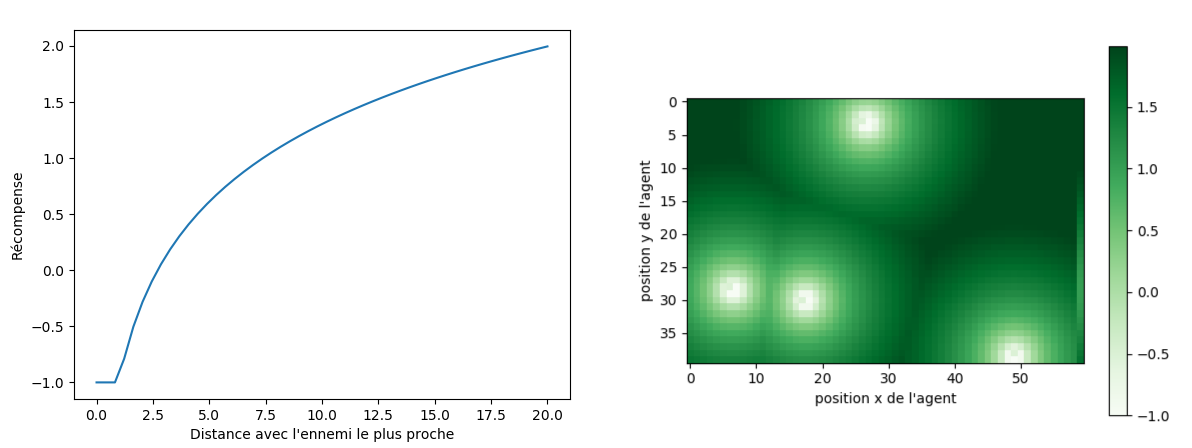
\includegraphics[scale=0.4]{ressources/reward_function_avoid_ennemies.png}
   \caption{Eviter ennemis: récompenses}
   \end{figure} 
   
  \par Ci-dessous, les histogrammes de l'agent en train d'apprendre. Nous constatons que la distribution des actions s'est répartie entre les 9 actions possibles, et que les poids du réseau neuronal évolue. 
  
   \begin{figure}[!h]
   \center
   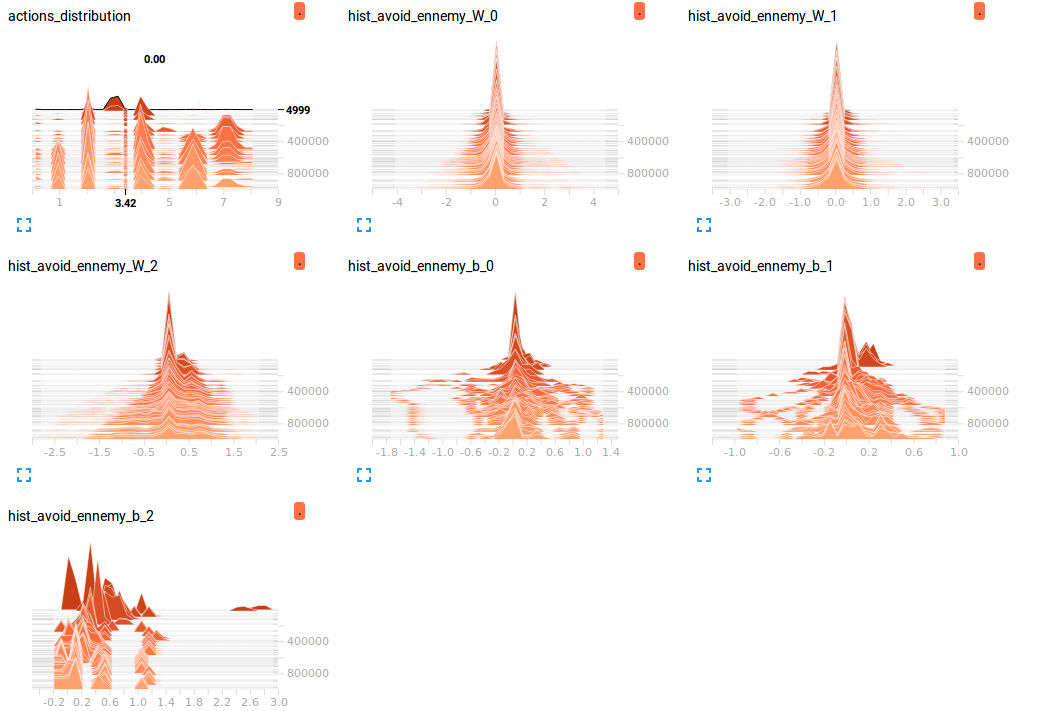
\includegraphics[scale=0.4]{ressources/reward_function_histograms_avoid_ennemies.png}
   \caption{Eviter ennemis: histogrammes}
   \end{figure} 

 \subsubsection{Attraper nourriture}
 
   \par La fonction récompense pour apprendre a attraper la nourriture dépend de la distance de l'agent avec la nourriture. Plus il est proche de celle-ci, plus la récompense sera élevée. Si l'endurance de l'agent tombe à 0, le jeu est terminé. L'agent reçoit à ce moment là un malus de $-5$. 
   
  \begin{lstlisting}[language=python]
def reward_function(world):
    if world.game_over:
        return - 5
    max_distance = 73
    return (1 - Direction.distance(world.agent, world.food) / max_distance) 
   \end{lstlisting}  
   
  
  \par Ci dessous à gauche la récompense en fonction de la distance de l'agent avec la nourriture. A droite, la récompense en fonction de la position de l'agent; la nourriture est dans la zone la plus verte. 
  
     \begin{figure}[!h]
   \center
   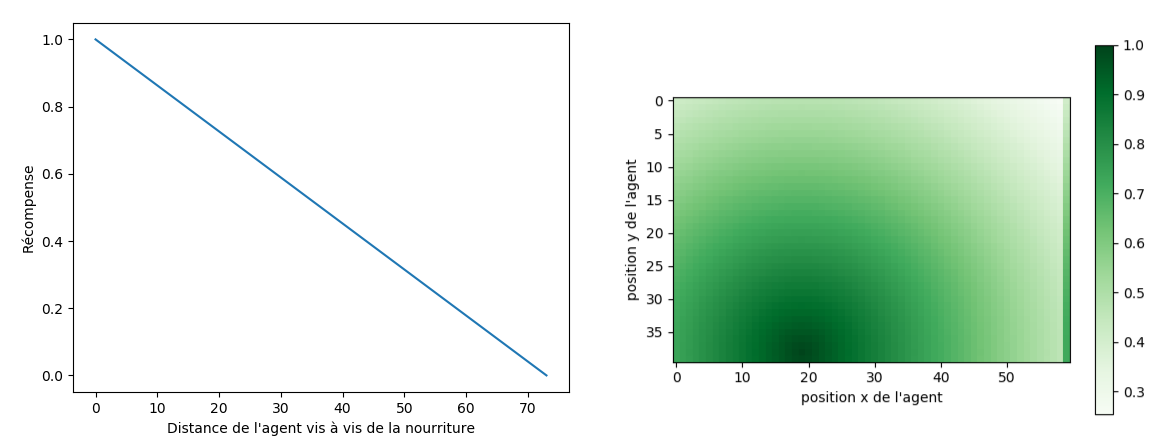
\includegraphics[scale=0.4]{ressources/reward_function_fetch_food.png}
   \caption{Attraper nourriture: récompense}
   \end{figure} 
   
  \par Ci dessous les histogrammes de l'agent en train d'apprendre à attraper la nourriture. 
        
   \begin{figure}[!h]
   \center
   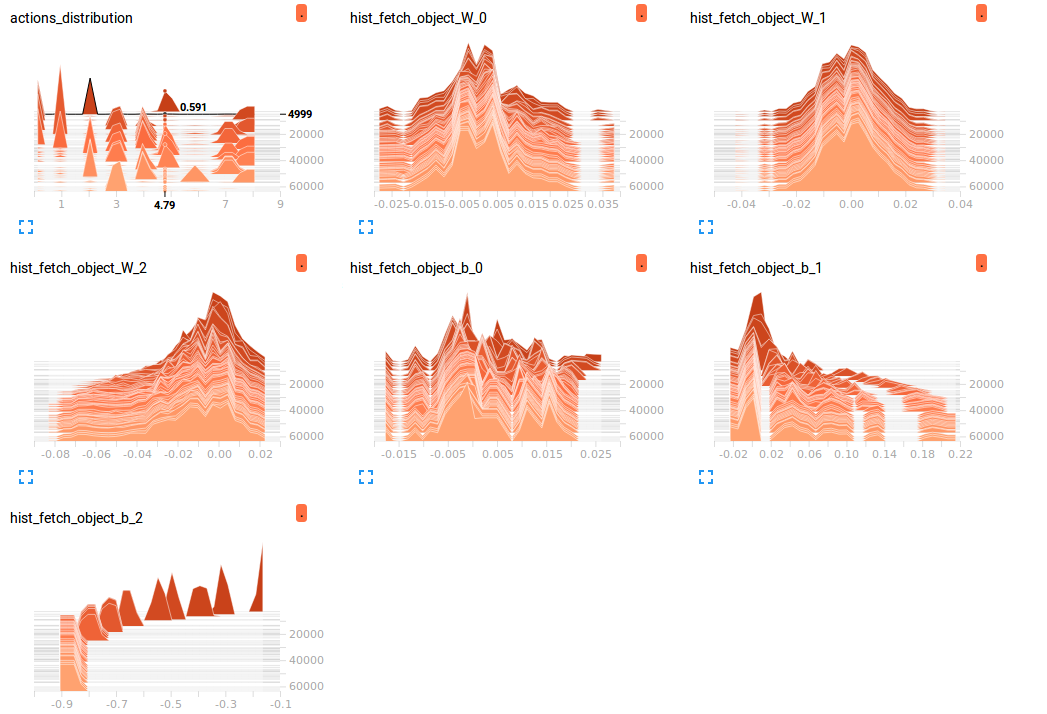
\includegraphics[scale=0.4]{ressources/reward_function_histograms_fetch_food.png}
   \caption{Eviter ennemis: histogrammes}
   \end{figure} 
   
   \subsubsection{Jouer au jeu complet}
   
   \par Enfin, lorsque l'agent doit apprendre à choisir quel réseau neuronal écouter entre le réseau "éviter les ennemis" et "attraper la nourriture", la même fonction que "attraper la nourriture" a été utilisée. Si l'endurance de l'agent tombe à zéro, le jeu est terminé. Si l'agent se fait attraper par un ennemi, le jeu est également terminé. Dans les deux cas, la fonction récompense attribue un malus de $-5$ si le jeu se termine. L'accent a été mis sur l'importance d'attraper de la nourriture.
   
   \section{Batch size}
   
   \subsection{Problème rencontré}
   
   \par Bien qu'une fonction récompense adéquate permet à l'agent d'apprendre, cela ne veut pas forcément dire que l'agent apprends dans des délais raisonnables. En effet, l'apprentissage pour éviter les ennemis prenait environ 14 jours avant d'arriver à un résultat médiocre. Afin d'accélérer le processus d'apprentissage, nous avons essayé d'augmenter la taille de l'échantillon (\textit{batch size}) avec lequel l'agent apprenait. Pour rappel, lorsque l’expérience de l'agent est suffisamment grande, la mise à jour des réseaux neuronaux est effectuée en prenant un échantillon aléatoire de la taille du paramètre \textit{batch size} sur l'expérience. 
   
   \par Au moment où l'apprentissage pour éviter les ennemis durait 14 jours, la taille de l'échantillon était de $32$, pioché sur une expérience de taille $50'000$. Ceci afin de s'assurer que l'apprentissage se fasse bien sur des échantillons suffisamment aléatoires. Nous avons donc tenté d'augmenter la taille de l'échantillon à $32'000$ pour sur une expérience de taille $50'000'000$ (en gardant la même proportion aléatoire), en espérant que l'agent apprendre plus rapidement en fonction de la taille de l'échantillon. \\
   Malheureusement, cela a empiré la durée de l'apprentissage. Ci dessous le graphique du score en fonction du nombre d'épisodes lors de l'apprentissage à éviter les ennemis. En bleu, le score pour un échantillon de taille $32$, en orange un échantillon de taille $32'000$.
   
   \begin{figure}[!h]
   \center
   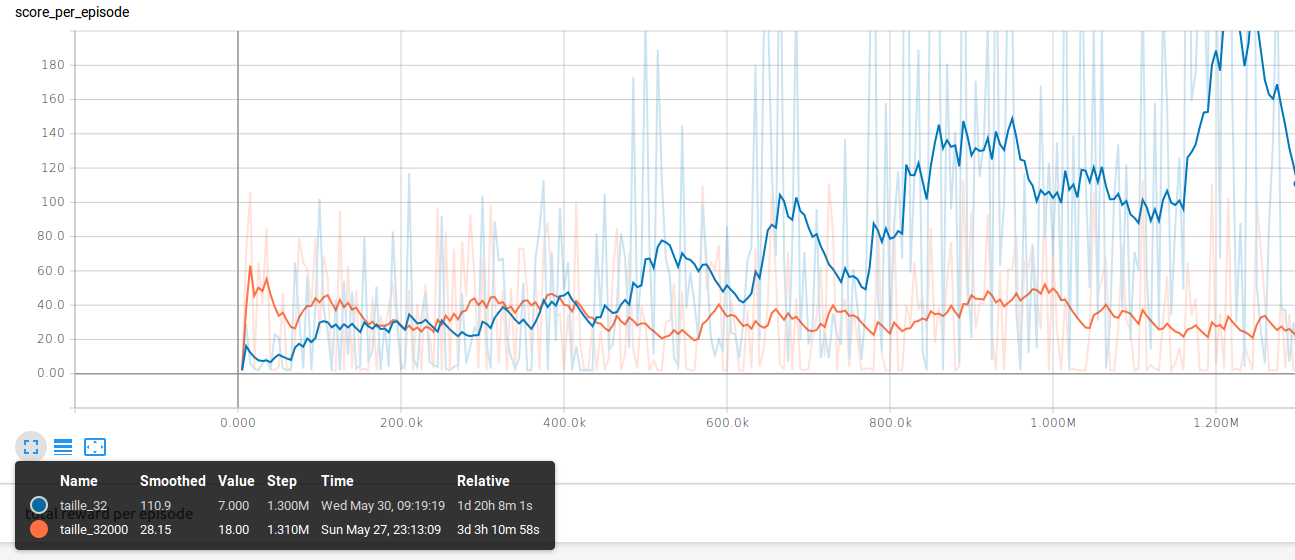
\includegraphics[scale=0.4]{ressources/batch_size.png}
   \caption{Score par épisode avec deux tailles d'échantillons}
   \end{figure} 
   
   \subsection{Explication}
   
   \par Comme bien souvent, la conclusion nous a paru évidente qu'une fois avoir effectué les tests. Pour un échantillon de taille $32$ et d’expérience $50'000$, l'agent effectue $50'000$ actions avant d'ajuster son réseau neuronal. Cela veut dire qu'il doit attendre $50'000$ actions avant d'améliorer son comportement. Avec un échantillon de taille $32'000$ et d'expérience de taille $50'000'000$, l'agent doit attendre d'avoir effectué $50'000'000$ actions avant d'améliorer son comportement; l'apprentissage se fait donc beaucoup plus lentement. 
   
   \par A l'heure où ces lignes sont écrites, nous nous rendons compte que l'importance de cette section n'est peut être pas la taille de l'échantillon, mais de la taille de l’expérience avant d'effectuer la mise à jour du réseau neuronal. Il semblait important au moment des tests de garder un proportion $\frac{\text{taille échantillon}}{\text{taille expérience}}$ suffisamment basse pour garantir l'homogénéité des échantillons utilisés lors de la mise à jour du réseau neuronal. Il doit cependant y avoir un juste milieu concernant ces paramètres. 
   
   \section{Entrées des réseaux neuronaux et discount factor $\gamma$}
   
   \par Le premier paramètre déterminant la vitesse d'apprentissage et de son efficacité fut de choisir adéquatement les données fournies au réseau neuronaux pour représenter l'état de l'environnement. Lorsque l'apprentissage pour éviter les ennemis durait 14 jours, les données fournies au réseau neuronal étaient la position de l'agent et la position des ennemis. La vitesse et l’efficacité de l'apprentissage ont drastiquement augmenté lorsque nous avons fourni les trois dernières positions de l'agent et les 3 dernières positions des ennemis. \\
   Cet ajout permet probablement au réseau neuronal d'enregistrer non seulement la position des acteurs de l'environnement, mais également leurs directions, ce qui permet d'anticiper plus facilement quelle est la meilleure action à effectuer. 
   
   \par Cet ajout n'a cependant pas été le seul facteur déterminant. Le choix du \textit{discount factor} $\gamma$ est également décisif. Pour rappel, l'hyper-paramètre \textit{discount factor} $\gamma$ représente en quelque sorte la valeur d'une récompense future, c'est à dire d'une récompense probable dans des états futurs (cf Chapitre 2, section "Notion de base"). Avec $\gamma = 1$, la valeur d'un état menant à une récompense future est la même qu'un état attribuant cette même récompense. Une valeur $\gamma = 0$, la récompense future ne nous intéresse pas, et seule la récompense immédiate a de l'importance. Le \textit{discount factor} $\gamma$ répond en quelque sorte à la question: est-ce qu'il vaut mieux accepter une récompense de 1 immédiatement, ou attendre une récompense probable de 100 future? 
   
   \par Ci dessous le graphique représentant le score par épisode en fonction du nombre d'épisodes vécus, pour l'apprentissage à "éviter les ennemis". En choisissant un $\gamma = 0.8$ et en fournissant les trois dernières positions de l'agent et ennemis au réseau neuronal, la durée de l'apprentissage a pu être réduit à quatre / cinq jours au lieu de 14 jours. 
   
   \begin{figure}[!h]
   \center
   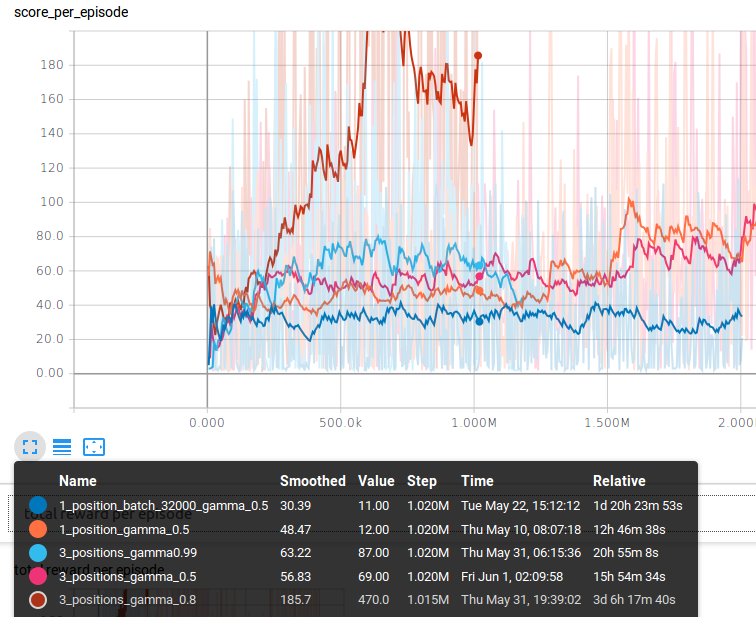
\includegraphics[scale=0.5]{ressources/input_size_gamma.png}
   \caption{Score par épisode avec en fonction du nombre d'épisodes vécus}
   \end{figure} 
   
   \section{Learning rate}
   
   \par Le dernier paramètre décisif dans la vitesse d'apprentissage fut de choisir un "learning rate" $\alpha$ plus élevé. Pour rappel, le poids des réseaux neuronaux sont ajustés de la manière suivante (cf chapitre 2, section 2.3.2: Valeur d’un état avec Q(s,a)). 
   
   $$W = W + \alpha \frac{dJ(Y,T)}{dW}$$
   
   \par L'idée du paramètre \textit{learning rate} $\alpha$ est de mettre à jour le poids $W$ petit à petit, afin d'éviter une mise à jour trop brusque, faussant l'apprentissage. Jusqu'ici, la valeur du learning rate était de $\alpha = 0.01$. Choisir $\alpha$ trop petit rend l'apprentissage plus long, mais choisir $\alpha$ trop élevé peut totalement casser l'apprentissage. Une valeur dix fois plus élevée $\alpha = 0.1$ pour l'apprentissage à éviter les ennemis et attraper la nourriture a permis de réduire la durée de l'apprentissage à 72 heures maximum au lieu de quatre / cinq jours maximum. Pour l'apprentissage à jouer au jeu complet, la valeur $\alpha = 0.1$ a cependant cassé l'apprentissage, et la valeur de $\alpha = 0.01$ a été gardée. 
   
  \section{Hyper-paramètres finaux}
  
  \par Pour terminer ce chapitre, voici la liste des hyper-paramètres utilisés pour chacun des scripts \textbf{trainer\_*.py}. Bien que les plus importants aient été décrits dans les sections précédentes, il parait important de signaler que les apprentissages tel qu'ils ont été décrit jusqu'ici n'auraient pas été les mêmes sans la combinaison de tous les hyper-paramètres à prendre en compte dans l'apprentissage par renforcement. Le seul paramètre qui n'est pas décrit dans cette section est le choix de la fonction de récompense, vu qu'elle a été décrite dans une section précédente. 
  
   \textbf{Hyper-paramètres communs aux 3 scripts:}   
   \begin{eqnarray}
   \epsilon \text{ (probabilité d'action aléatoire) } &=& 0.1 \text{ (constante)} \\
   \text{fréquence de la mise à jour du TNetwork } &=& 10'000 \\
   \text{taille experience } &=& 50'000 \\
   \text{batch size } &=& 32 
   \end{eqnarray}
   
   \textbf{Script éviter les ennemis:}
   \begin{eqnarray}
   \alpha \text{ (learning rate) } &=& 0.1 \\
   \gamma \text{ (discount factor) } &=& 0.8 \\
   \text{ input adapter } &=& \text{ 3 dernières position de l'agent et ennemis}
   \end{eqnarray}   
   
   \begin{figure}[!h]
   \center
   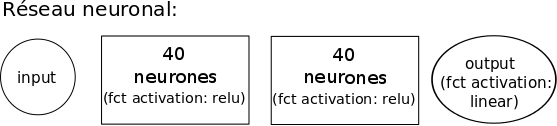
\includegraphics[scale=0.45]{ressources/nn_model.png}
   \caption{Architecture réseau neuronal utilisé}
   \end{figure} 
   
   
   \textbf{Script attraper la nourriture:}
   \begin{eqnarray}
   \alpha \text{ (learning rate) } &=& 0.1 \\
   \gamma \text{ (discount factor) } &=& 0.5 \\
   \text{ input adapter } &=& \text{ position agent et position nourriture}
   \end{eqnarray}   
   
   \textbf{Script jouer au jeu complet:}
   \begin{eqnarray}
   \alpha \text{ (learning rate) } &=& 0.01 \\
   \gamma \text{ (discount factor) } &=& 0.5 \\
   \text{ input adapter } &=& \text{ endurance, distance ennemis et nourriture}
   \end{eqnarray}   
  
  \chapter{Conclusion}
  
  \section{Difficultés}
  
  \par Pour terminer, il parait important de relever les difficultés rencontrées lors de l'étude de l'apprentissage par renforcement. Le champ de celui-ci est vaste et est encore sujet à de nombreuses recherches. Il évolue d'années en années, et de nouveaux algorithmes voient le jour régulièrement. Il n'est évident de se plonger dans cette branche du machine learning tant les ressources sont diverses et pointues, et la théorie est bien souvent loin d'algorithmes concrets à reproduire chez soi. \\
  Par ailleurs, le nombre important d'hyper-paramètres à ajuster rend l'implémentation difficile lorsque l'on cherche à résoudre un problème donné, bien que l'architecture créé pour cela aie été développée sans erreurs. \\
  Enfin, le temps d'apprentissage est également une des principales contraintes. Si la compilation de certains programmes peut durer des heures, il n'est pas rare de devoir attendre des semaines afin de voir si l'agent apprend comme prévu. 
  
  \section{Perspectives}
  
   \par Cela reste néanmoins un sujet passionnant, d'actualité, qui mérite d'être approfondi. Avec l'avancée d'années en années de la recherche sur ce sujet, qui sait de quoi sera faite la technologie de demain. Il me parait important de suivre l'évolution de celui-ci pour pouvoir y garder un avis critique. 

  \subsection{Nouvel environnement}  
  
  \par Si le temps me permettais d'améliorer ce travail de bachelor, je commencerais par changer d'environnement: l'environnement utilisé s'est avéré inapproprié. En effet, bien qu'il aie été possible d'enseigner à l'agent des tâches spécifiques telles qu'éviter des ennemis ou attraper de la nourriture, enseigner à l'agent à évoluer dans l'environnement complet en utilisant uniquement deux compétences n'est pas adaptée. Si l'ennemi le plus proche de l'agent et la nourriture se trouvent en bas à droite de l'agent, l'agent n'a pas la possibilité de choisir une action convenable afin d'éviter l'ennemi et de se diriger vers la nourriture. 

   \begin{figure}[!h]
   \center
   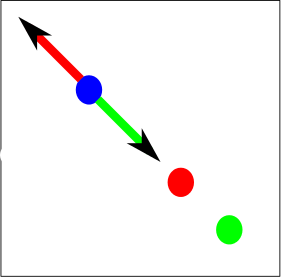
\includegraphics[scale=0.3]{ressources/percpective.png}
   \caption{Situation non adaptée à l'architecture choisie}
   \end{figure} 

  
  \par L'exemple ci-dessus illustre ces propos. Dans cet état, le réseau neuronal "éviter ennemis" recommande de se diriger en haut à gauche, alors que le réseau  "attraper nourriture" recommande de se diriger en bas à droite. Le réseau "jouer au jeu complet" devrait choisir entre une de ces deux actions recommandées, et n'a pas possibilité de choisir une action intermédiaire. 
  
  \par Un environnement plus adapté à l'architecture de ce travail de bachelor serait par exemple un corps dans lequel l'agent doit apprendre à se mouvoir. 
  
   \begin{figure}[!h]
   \center
   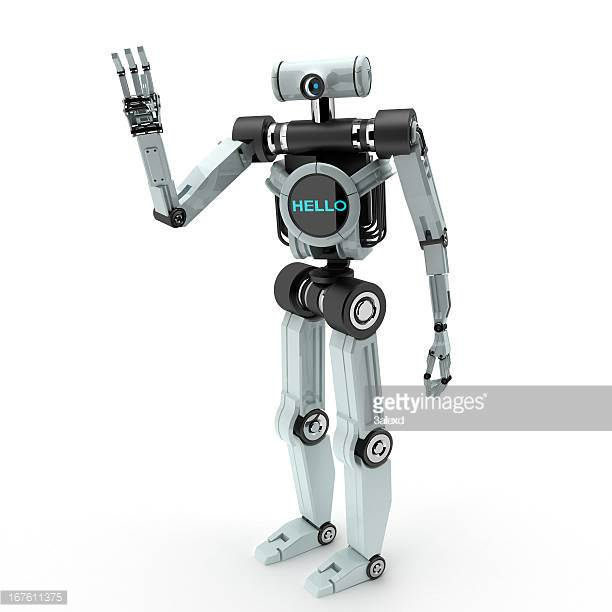
\includegraphics[scale=1]{ressources/robot.jpg}
   \caption{Nouvel environnement}
   \end{figure} 
   
   \par Nous pourrions par exemple envisager un réseau neuronal pour apprendre à marcher, un autre pour apprendre à se relever lorsque le corps tombe, un troisième pour apprendre à attraper un objet à portée de main, et le dernier réseau pour apprendre à jongler entre les réseaux neuronaux. Les réseaux neuronaux ne seraient pas en contradictions contrairement à l'environnement de ce projet de bachelor. 
   
  \subsection{Nouvel algorithme}
  
  \par Un autre élément que je changerais est l'algorithme d'apprentissage par renforcement utilisé. L'algorithme "Deep Q-Network" utilisé dans ce travail de bachelor date de 2015 est à présent presque devenu un "cas d'école". Le désavantage de celui-ci est qu'il est "lent" d'apprentissage: il a pour but de diminuer l'erreur de Bellman (optimiser l'équation de Bellman) en n'ajustant que les valeurs pour les actions que l'agent a effectuées. D'autres algorithmes plus performants ont depuis vu le jour, comme les algorithmes "actor / critic": au lieu d'utiliser un QNetwork et un TNetwork, l'on peut par exemple utiliser un réseau neuronal ayant pour but d'estimer la meilleure action dans un état donné (actor), et un autre réseau ayant pour but d'estimer "l'erreur" du réseau "actor". Le réseau "actor" ne se mettrait pas à jour en fonction des récompenses reçues, mais uniquement en fonction des prévisions effectuées par le réseau "critic". L'avantage est que l'acteur mettrait à jour l’entièreté des valeurs de Q(s,a), et non uniquement des actions effectuées par l'agent. Le réseau "critic" se mettrait à jour en fonction des récompenses reçues en fonction de chaque état rencontré. Cette séparation (semble t'il) rend l'apprentissage plus générique et efficace. 
  
  \chapter{Annexes}
  
  \section{Installation}
  
  \par Les pré-requis sont \textbf{python3}, \textbf{pip}, \textbf{python3-tk} et \textbf{git}
  
  \begin{lstlisting}[language=bash]
# télécharger le projet
git clone https://github.com/Eldorico/deep-q-network-bachelor.git
cd deep-q-network-bachelor

# créer un environnement python virtuel dans le dossier
pip install virtualenv
virtualenv virtual_env_folder

# activer l'environnement virtuel
source virtual_env_folder/bin/activate

# installer les dépendances
pip install tensorflow
pip install gym
pip install pygame
  \end{lstlisting}  
  
 \section{Jouer soi-même au jeu}
  \begin{lstlisting}[language=bash]
# activer l'environnement virtuel
source virtual_env_folder/bin/activate

# configurer le fichier src/world.py en fonction du besoin
# (dans la partie __main__)
# puis lancer l'environnement
cd src
python world.py

# s'ouvriront 2 fenetres: une petite noire, et l'autre avec le jeu:
# avoir le focus sur la fenetre noire, 
# et jouer avec les fleches directionnelles
  \end{lstlisting}  
  
 \section{Voir l'agent évoluer}
  \begin{lstlisting}[language=bash]
# activer l'environnement virtuel
source virtual_env_folder/bin/activate

# se déplacer ds dossier src
cd src 

# executer l'un des scripts suivants
# python see_avoid_ennemies_in_action.py
# python see_fetch_object_in_action.py
# python see_play_game_in_action.py
  \end{lstlisting}  

\section{Entraîner l'agent depuis zéro}
\begin{lstlisting}[language=bash]
# activer l'environnement virtuel
source virtual_env_folder/bin/activate

# se déplacer ds dossier src
cd src 

# lancer le script pour apprendre à éviter les ennemis
python trainer_avoid_ennemies.py
# attendre 72 heures. Si le script n'est pas terminé, arrêter avec ctrl+c

# lancer le script pour apprendre à attraper la nourriture
python trainer_fetch_object.py
# attendre 72 heures. Si le script n'est pas terminé, arrêter avec ctrl+c

# copier les réseaux enregistrés dans le dossier un dossier play_game
mkdir ../tmp_saves/play_game
cp ../tmp_saves/avoid_ennemies/* ../tmp_saves/play_game
cp ../tmp_saves/food/* ../tmp_saves/play_game

# lancer le script pour apprendre à jouer le jeu complet
python trainer_play_game.py
# attendre 72 heures. Si le script n'est pas terminé, arrêter avec ctrl+c

  \end{lstlisting}  

\end{document}
